\chapter{Artificial Neural Networks}\label{ch:neural_networks}

Artificial neural networks (\gls{ANN}) represent one of the earliest and most successful approaches to biologically inspired computation. Their development began in 1943 when Warren McCulloch and Walter Pitts proposed the first formal mathematical model of an artificial neuron~\citep{McCullochPitts1943}, establishing the conceptual foundations that endure to this day.

The central motivation of \gls{ANN} is to emulate, in a simplified manner, the information processing of biological neurons. These specialized cells receive input signals, integrate them through complex electrochemical processes, and generate output responses that propagate through interconnected networks. Crucially, biological neurons exhibit synaptic plasticity, adapting their responses based on experience and enabling learning from examples.

This analogy with the processing mechanisms of the human brain has motivated decades of research in artificial intelligence, seeking to develop computational systems capable of learning and adapting in a manner similar to biological systems. In this chapter we will examine the mathematical foundations of \gls{ANN}, from the individual neuron to modern deep architectures.

\section{Artificial Neuron}\label{sec:neurona_artificial}

\begin{figure}[h]
	\centering
	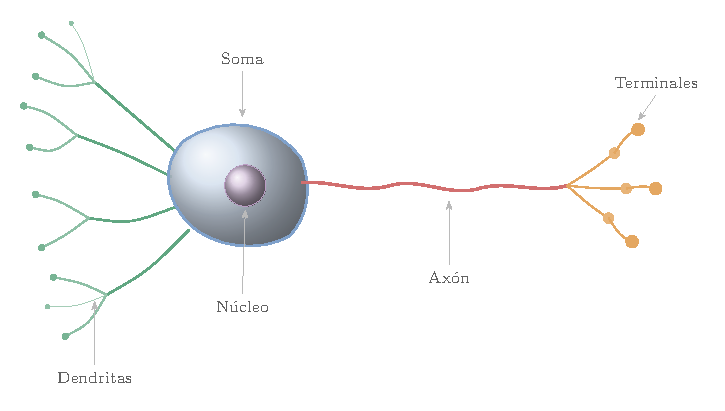
\includegraphics[width=0.6\textwidth]{images/neuron_biological}
	\caption[Diagram of a biological neuron]{Diagram of a biological neuron showing dendrites (inputs), soma (cell body), and axon (output). This structure inspired the McCulloch-Pitts mathematical model.}
	\label{fig:neuron}
\end{figure}

The McCulloch-Pitts model established the conceptual foundations by abstracting the behavior of a biological neuron (\autoref{fig:neuron}) into simple mathematical terms. In the nervous system, neurons receive electrochemical signals from other cells through dendrites and synaptic connections. These signals are integrated in the cell soma, and if the weighted sum exceeds a critical depolarization threshold, the neuron generates an action potential that propagates through the axon toward other neurons.

Inspired by this mechanism, an artificial neuron constitutes a mathematical model that:
\begin{enumerate}
	\item Receives multiple numerical input signals
	\item Weights them through adjustable parameters (synaptic weights)
	\item Applies a nonlinear activation function that models the firing threshold
	\item Produces an output signal that can serve as input to other neurons
\end{enumerate}

It is important to recognize that real biological neurons exhibit a complexity that goes far beyond this initial abstraction. Neuronal processes involve complex temporal dynamics, specific chemical neurotransmitters, time-dependent synaptic plasticity, and intricate three-dimensional dendritic architectures. Nevertheless, the simplification of the McCulloch-Pitts model has proved to be extraordinarily fruitful, providing the conceptual basis for the development of modern \gls{ANN}.

\subsection{Mathematical formulation}

The standard mathematical model of an artificial neuron can be formulated as a function that maps an input vector \(\mathbf{x} = (x_1, x_2, \ldots, x_n)^T\) to a scalar output \(y\). The fundamental operation consists of:

\begin{equation}
	y = \sigma\left(\sum_{i=1}^{n} w_i x_i + b\right)
	\label{eq:neuron}
\end{equation}

where:
\begin{itemize}
	\item \(\mathbf{w} = (w_1, w_2, \ldots, w_n)^T\) are the synaptic weights that modulate the importance of each input
	\item \(b\) is the bias or activation threshold
	\item \(\sigma\) is the nonlinear activation function
\end{itemize}

The activation function \(\sigma\) plays a fundamental role by introducing the essential nonlinearity that allows neural networks to approximate complex functions and capture nonlinear relationships in the data. The synaptic weights \(\mathbf{w}\) and the bias \(b\) constitute the adjustable parameters of the model. These are updated during the training process to approximate the desired target function.

\subsubsection{Spiking Neural Networks}

It is important to mention that this classical formulation, although extremely successful, represents a simplified abstraction of neuronal behavior. There exist alternative models that are closer to biology, such as \textbf{Spiking Neural Networks} or \gls{SNN}, considered the ``third generation'' of neural networks \citep{Maass1997spiking}. Unlike the classical model where the output is a continuous value, \glspl{SNN} process information through discrete pulses (spikes) that propagate over time, thus capturing the temporal dynamics inherent to biological neurons. These networks use models such as \textit{Integrate-and-Fire} or \textit{Hodgkin-Huxley}, where the neuron accumulates membrane potential until reaching a threshold and emitting a spike. \glspl{SNN} offer significant computational advantages in terms of energy efficiency and are especially promising for neuromorphic hardware \citep{Tavanaei2018deep}. However, for the purposes of this work, we will focus on the classical artificial neuron model described above.

\subsubsection{Formal definition}

To establish a rigorous mathematical framework for this work, we first formalize the concept of activation function and, subsequently, that of artificial neuron.

\begin{definition}[Activation function]\label{def:funcion_activacion}
	An \textit{activation function} is a function $\sigma: \mathbb{R} \to \mathbb{R}$ that satisfies the following properties:
	\begin{itemize}
		\item \textbf{Nonlinearity}: $\sigma$ is not an affine map,
		\item \textbf{Continuity}: $\sigma$ is continuous,
		\item \textbf{Differentiability almost everywhere}: $\sigma$ is differentiable except possibly on a set of Lebesgue measure zero\footnote{A set $A \subset \mathbb{R}$ has Lebesgue measure zero if it can be covered by intervals whose total length is arbitrarily small. See Definitions~\ref{def:medida_lebesgue} and \ref{def:casi_por_doquier} for the formal definition.}.
	\end{itemize}
\end{definition}

These properties ensure that $\sigma$ can introduce the nonlinearities necessary for the expressive capacity of the network, while allowing the computation of gradients for training through backpropagation. \autoref{tab:funciones_activacion} summarizes the main activation functions used in practice along with their most relevant properties, and \autoref{subsubsec:funciones_activacion_capas} describes each of them in detail.

\begin{definition}[Artificial neuron]\label{def:neurona_artificial}
	Let $n \in \mathbb{N}$ and let $\sigma: \mathbb{R} \to \mathbb{R}$ be an activation function. For each $\theta = (\mathbf{w}, b) \in \mathbb{R}^{n+1}$ with $\mathbf{w} \in \mathbb{R}^n$ (weights) and $b \in \mathbb{R}$ (bias), an \textit{artificial neuron} is a function $f_{\theta}: \mathbb{R}^n \to \mathbb{R}$ expressed as the composition of an affine map with an activation function:
	\begin{equation}
		f_{\theta}(\mathbf{x}) = \sigma \circ T_{\theta}(\mathbf{x}) = \sigma\Big( \langle \mathbf{w}, \mathbf{x} \rangle + b \Big)
		\label{eq:neuron_formal}
	\end{equation}
	where $T_{\theta}: \mathbb{R}^n \to \mathbb{R}$ is the \textit{affine map} defined by
	\[
	T_{\theta}(\mathbf{x}) = \langle \mathbf{w}, \mathbf{x} \rangle + b.
	\]
\end{definition}

The set of parameters $\theta$ is trainable, which means that during the learning process it is adjusted to minimize a loss function. Thus, an artificial neuron defines a \textit{family of functions} $\{f_{\theta} : \theta \in \mathbb{R}^{n+1}\}$ parameterized by the weights and the bias.

\autoref{fig:neurona_artificial} illustrates the structure of an artificial neuron, showing the flow from the weighted inputs to the activated output.

\begin{figure}[h]
\centering
\begin{tikzpicture}[
    node distance=0.8cm,
    input/.style={circle, draw, minimum size=0.6cm, fill=gdlblue!15},
    weight/.style={rectangle, draw, minimum width=0.6cm, minimum height=0.4cm, fill=gdlgray!15, font=\scriptsize},
    sum/.style={circle, draw, minimum size=0.8cm, fill=gdlyellow!20},
    activation/.style={rectangle, draw, rounded corners, minimum width=0.8cm, minimum height=0.6cm, fill=gdlgreen!20},
    output/.style={circle, draw, minimum size=0.6cm, fill=gdlred!15},
    arrow/.style={->, thick, >=stealth}
]

% Entradas
\node[input] (x1) at (0, 1.5) {$x_1$};
\node[input] (x2) at (0, 0) {$x_2$};
\node[input] (xn) at (0, -1.5) {$x_n$};
\node at (0, -0.75) {$\vdots$};

% Pesos
\node[weight] (w1) at (1.5, 1.5) {$w_1$};
\node[weight] (w2) at (1.5, 0) {$w_2$};
\node[weight] (wn) at (1.5, -1.5) {$w_n$};

% Nodo sumador
\node[sum] (suma) at (3.5, 0) {$\sum$};
\node[below=0.1cm of suma, font=\scriptsize] {$+b$};

% Función de activación
\node[activation] (sigma) at (5.5, 0) {$\sigma$};

% Salida
\node[output] (y) at (7, 0) {$y$};

% Conexiones
\draw[arrow] (x1) -- (w1);
\draw[arrow] (x2) -- (w2);
\draw[arrow] (xn) -- (wn);
\draw[arrow] (w1) -- (suma);
\draw[arrow] (w2) -- (suma);
\draw[arrow] (wn) -- (suma);
\draw[arrow] (suma) -- node[above, font=\scriptsize] {$z$} (sigma);
\draw[arrow] (sigma) -- (y);

% Etiquetas de fases
\node[above=1.5cm of x1, font=\small\bfseries] {Inputs};
\node[above=0.3cm of w1, font=\small\bfseries] {Weights};
\node[above=0.5cm of suma, font=\small\bfseries] {Sum};
\node[above=0.5cm of sigma, font=\small\bfseries] {Activation};

\end{tikzpicture}
\caption[Structure of an artificial neuron]{Structure of an artificial neuron. The inputs $x_i$ are multiplied by weights $w_i$, summed together with the bias $b$, and the result $z = \sum w_i x_i + b$ is transformed by the activation function $\sigma$ to produce the output $y = \sigma(z)$.}
\label{fig:neurona_artificial}
\end{figure}

The nonlinearity of $\sigma$ is crucial: the composition of multiple affine maps remains an affine map, so that without nonlinear activation functions, a deep neural network with multiple layers would be equivalent to a single linear transformation, losing all its expressive capacity. It is this nonlinearity that allows neural networks to approximate arbitrarily complex functions, as established by the universal approximation \autoref{thm:aproximacion_universal} (see \autoref{sec:aproximacion_universal}).

\subsubsection{Desirable properties of activation functions}

Although \autoref{def:funcion_activacion} establishes the minimum properties necessary for a function to serve as an activation function, in practice it is desirable that it satisfy additional properties that facilitate training and improve the behavior of neural networks. Below we present a detailed analysis of these desirable properties.

\begin{definition}[Boundedness or controlled growth]\label{prop:acotacion_activacion}
	An activation function $\sigma: \mathbb{R} \to \mathbb{R}$ has \textit{controlled growth} if it satisfies one of the following conditions:
	\begin{enumerate}
		\item \textbf{Boundedness}: There exists $M > 0$ such that $|\sigma(z)| \leq M$ for all $z \in \mathbb{R}$.
		\item \textbf{Linear growth}: There exist constants $C_1, C_2 > 0$ such that $|\sigma(z)| \leq C_1|z| + C_2$ for all $z \in \mathbb{R}$.
	\end{enumerate}
\end{definition}

This property is crucial for numerical stability during training. The first condition (boundedness) guarantees that activations remain within a finite range regardless of the magnitude of the input, preventing any numerical overflow. The second condition (linear growth) is more permissive: it allows activations to grow, but at a rate no greater than that of the input itself. In both cases, the explosion of values during forward propagation is prevented, which otherwise could cause numerical overflows or excessively large gradients. \autoref{tab:funciones_activacion} shows that the usual activation functions satisfy one or the other condition; for detailed descriptions of each function, see \autoref{subsubsec:funciones_activacion_capas}.

\begin{definition}[Monotonicity]\label{prop:monotonia_activacion}
	A function $\sigma: \mathbb{R} \to \mathbb{R}$ is \textit{monotonic} (increasing) if for any $z_1, z_2 \in \mathbb{R}$ with $z_1 < z_2$ it holds that:
	\[
	\sigma(z_1) \leq \sigma(z_2)
	\]
\end{definition}

Monotonicity provides three fundamental advantages:
\begin{enumerate}
	\item \textbf{Order preservation}: Activations maintain the relative order of the inputs, facilitating interpretability.
	\item \textbf{Uniqueness of local optima}: In combination with convexity of the loss function, it simplifies the optimization landscape.
	\item \textbf{Smoothness of the loss surface}: It reduces the presence of spurious local minima in the parameter space.
\end{enumerate}

Most classical activation functions are monotonic (see \autoref{subsubsec:funciones_activacion_capas}). However, monotonicity is not a necessary condition for good empirical performance: there exist non-monotonic activation functions that exhibit competitive results in practice, which suggests that the theoretical advantages of monotonicity may be offset by other favorable properties.

\begin{definition}[Zero-centered]\label{prop:zero_centered}
	An activation function $\sigma: \mathbb{R} \to \mathbb{R}$ is \textit{zero-centered} if it satisfies:
	\begin{enumerate}
		\item $\sigma(0) = 0$ or $\sigma(0) \approx 0$
		\item It is symmetric with respect to the origin: $\sigma(-z) = -\sigma(z)$ for all $z \in \mathbb{R}$ (odd function)
	\end{enumerate}
\end{definition}

This property significantly accelerates the convergence of training. When activations are zero-centered, the gradients have a mean close to zero, which avoids systematic biases in the weight updates.

When an activation function does not satisfy this property (for example, if its range is not centered at the origin, if $\sigma(0) \neq 0$), the outputs of each layer present a systematic bias. This causes all the gradients with respect to the weights of the same layer to have the same sign, causing the ``zigzagging'' phenomenon during gradient descent: the parameter updates oscillate between orthogonal directions instead of converging directly toward the optimum.

\begin{definition}[Non-saturating gradient]\label{prop:gradiente_no_saturante}
	An activation function $\sigma: \mathbb{R} \to \mathbb{R}$ has a \textit{non-saturating gradient} if there exists $\delta > 0$ and a set $S \subseteq \mathbb{R}$ of infinite measure such that:
	\[
	|\sigma'(z)| \geq \delta \quad \text{for all } z \in S
	\]
\end{definition}

This property is fundamental to avoid the \textit{vanishing gradient} problem, one of the main obstacles in training deep networks (see the formal analysis in \autoref{subsubsec:backpropagation}).

\begin{corollary}
Every bounded activation function with horizontal asymptotes necessarily saturates.
\end{corollary}

\begin{proof}
If $\lim_{z \to \pm\infty} \sigma(z) = c_{\pm}$ with $c_+, c_-$ finite, then $\lim_{z \to \pm\infty} \sigma'(z) = 0$. For any $\delta > 0$, there exists $M > 0$ such that $|\sigma'(z)| < \delta$ for all $|z| > M$, so that the set $\{z : |\sigma'(z)| \geq \delta\} \subseteq [-M, M]$ has finite measure. By \autoref{prop:gradiente_no_saturante}, $\sigma$ cannot have a non-saturating gradient and, therefore, necessarily saturates.
\end{proof}

When $|z|$ is large, $|\sigma'(z)| \approx 0$, which causes the gradients to become exponentially small in deep layers during backpropagation. Mathematically, if we consider a network with $L$ layers where each layer has a saturated activation, the gradient of the loss with respect to the weights of the first layers will be proportional to $\prod_{\ell=1}^{L} \sigma'(z^{(\ell)})$, which can become numerically zero.

A function that maintains $|\sigma'(z)| \geq \delta > 0$ on a set of infinite measure allows the gradient to flow without attenuation through multiple layers. The optimal case corresponds to functions whose derivative is constant equal to 1 on a half-line, which completely eliminates saturation in that active region and facilitates the training of very deep networks. Moreover, if one requires $|\sigma'(z)| > 0$ for all $z \in \mathbb{R}$ (that is, a strictly nonzero gradient over the entire domain), the risk that certain neurons stop contributing to learning (a phenomenon known as ``dead neurons'') is eliminated.

\autoref{fig:vanishing_gradient} (see \autoref{subsubsec:backpropagation}) visually illustrates how the gradient vanishes exponentially in deep networks with saturating activations, compared to the stable behavior of non-saturating activations.

\begin{definition}[Computational efficiency]\label{prop:eficiencia_computacional}
	An activation function is \textit{computationally efficient} if both $\sigma(z)$ and its derivative $\sigma'(z)$ can be evaluated in $O(1)$ time with basic arithmetic operations.
\end{definition}

In deep neural networks with millions of neurons, the activation function is evaluated billions of times during training. Therefore, its computational efficiency has a direct impact on the total training time.

Taxonomy by type of operation:
\begin{itemize}
	\item \textbf{Comparisons and selections} (functions defined piecewise through $\max$): They require only comparison and selection operations, which makes them extremely efficient on modern hardware.
	\item \textbf{Transcendental functions} (exponentials, logarithms): They are evaluated in $O(1)$ but with a significantly larger constant than the previous ones, as they require internal polynomial approximations.
	\item \textbf{Vector functions} (normalization over the entire output vector): They have $O(n)$ complexity in the dimension of the vector, since they require computing global statistics before normalizing each component.
\end{itemize}

Although all these categories are polynomial in complexity, the differences in constants are significant in practice. The computationally simplest activation functions allow deeper networks to be trained in less time, which has been a relevant factor in the widespread adoption of comparison-based activations.

\begin{definition}[Lipschitz continuity]\label{prop:lipschitz_continuidad}
	A function $\sigma: \mathbb{R} \to \mathbb{R}$ is \textit{Lipschitz continuous} if there exists a constant $L > 0$ (called the \textit{Lipschitz constant}) such that for any $z_1, z_2 \in \mathbb{R}$:
	\[
	|\sigma(z_1) - \sigma(z_2)| \leq L |z_1 - z_2|
	\]
\end{definition}

Lipschitz continuity is stronger than uniform continuity and provides quantitative control over how perturbations in the input propagate to the output. This has certain advantages in the training of neural networks:

\begin{enumerate}
	\item \textbf{Numerical stability}: Small changes in the weights produce bounded changes in the activations.
	\item \textbf{Gradient control}: If $\sigma$ is Lipschitz with constant $L$, then $|\sigma'(z)| \leq L$ almost everywhere (where the derivative exists).
	\item \textbf{Convergence guarantees}: Many convergence theorems for optimization algorithms assume Lipschitz continuity of the objective function.
\end{enumerate}

For activation functions that are differentiable almost everywhere, the Lipschitz constant can be computed as $L = \sup_{z} |\sigma'(z)|$. Bounded functions with horizontal asymptotes tend to have small Lipschitz constants (since their derivative vanishes at the extremes and reaches a moderate maximum), while functions with linear growth typically present $L = 1$. \autoref{tab:funciones_activacion} collects the concrete values for the most common activation functions.

It should be noted that a function can be Lipschitz continuous without being of class $C^1$: it suffices that it be continuous and have a bounded derivative almost everywhere. At points of non-differentiability, subgradients are used, which is sufficient for the gradient-based optimization algorithms employed in the training of neural networks.

The properties presented are not mutually exclusive, and the most successful activation functions in practice usually combine several of them. \autoref{tab:funciones_activacion} summarizes the properties of the most widely used activation functions.

\begin{table}[h]
\centering
\caption{Comparison of common activation functions}
\label{tab:funciones_activacion}
\begin{tabular}{@{}lccccc@{}}
\toprule
\textbf{Function} & \textbf{Formula} & \textbf{Range} & \textbf{Centered} & \textbf{Non-saturating} & \textbf{Lipschitz} \\
\midrule
Sigmoid & $\frac{1}{1+e^{-z}}$ & $(0,1)$ & No & No & $L=\frac{1}{4}$ \\
\addlinespace
Tanh & $\frac{e^z-e^{-z}}{e^z+e^{-z}}$ & $(-1,1)$ & Yes & No & $L=1$ \\
\addlinespace
ReLU & $\max(0,z)$ & $[0,\infty)$ & No & Yes ($z>0$) & $L=1$ \\
\addlinespace
Leaky ReLU & $\max(\alpha z,z)$ & $\mathbb{R}$ & No & Yes & $L=1$ \\
\addlinespace
Swish & $z \cdot \sigma(z)$ & $\approx(-0.3,\infty)$ & No & Partial & $L\approx 1.1$ \\
\bottomrule
\end{tabular}
\end{table}

\autoref{fig:activation_functions} graphically shows the most common activation functions together with their derivatives, allowing one to visualize the saturation zones and the behavior of the gradient.

\begin{figure}[htbp]
\centering
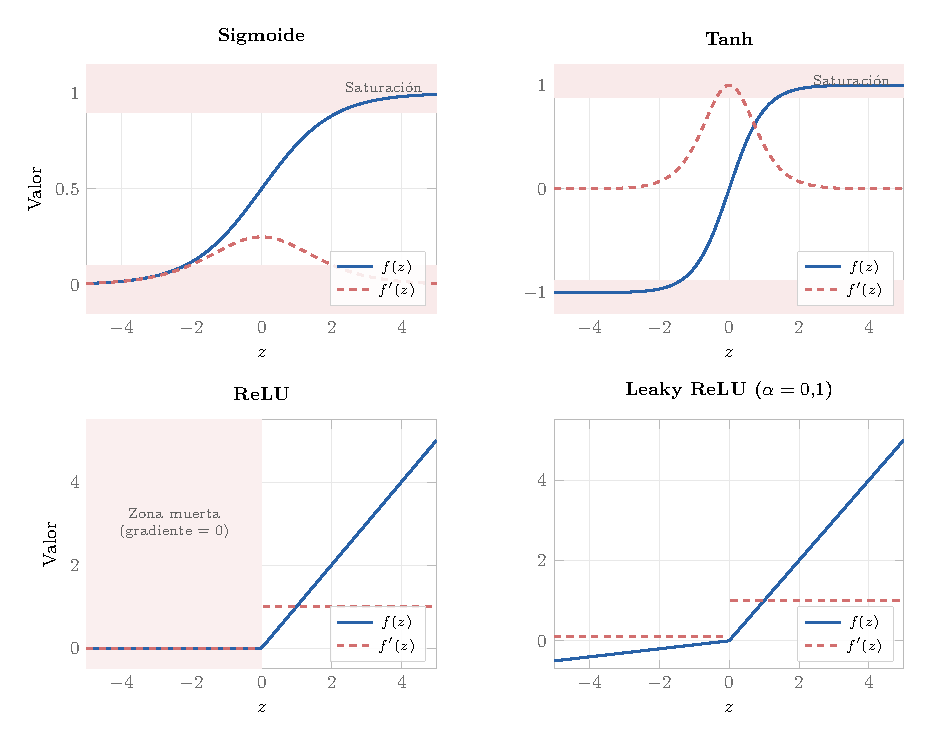
\includegraphics[width=0.95\textwidth]{images/activation_functions}
\caption[Plots of activation functions]{Common activation functions and their derivatives. The shaded zones indicate regions of saturation where the gradient tends to zero. Note how ReLU maintains a constant gradient for $z > 0$, while Sigmoid and Tanh saturate at the extremes.}
\label{fig:activation_functions}
\end{figure}

A fundamental theoretical result that justifies the use of activation functions with these properties is the \textbf{universal approximation theorem} (see \autoref{sec:aproximacion_universal}), which establishes that neural networks with a single hidden layer and appropriate activation functions can approximate any continuous function on a compact set with arbitrary precision. This theorem will be presented and proved in detail later in this chapter, together with the functional analysis preliminaries necessary for its complete understanding.

The choice of the appropriate activation function depends on the specific problem, the network architecture, and practical training considerations. In the following sections we will see how these properties influence architecture design.

\section{Data and its structure}\label{sec:datos_estructura}

In the previous section we defined the artificial neuron as a function that processes input data and generates output data. However, in this formulation we have not spoken about the information or the data that the neural network processes; we have not stopped to think about what the space $\mathbb{R}^n$ really represents. It is necessary to understand whether the data in the space $\mathbb{R}^n$ are simply numbers or whether there is some kind of relationship between them that contains relevant information.

This distinction is crucial. When we represent a $28 \times 28$ pixel image as a vector in $\mathbb{R}^{784}$, we are not dealing with $784$ independent values: each component corresponds to a specific pixel in a two-dimensional grid, and spatially neighboring pixels are naturally related. The grid structure is not arbitrary, but intrinsic to the nature of the image.

In this section we will formalize this distinction through two complementary conceptual frameworks that will allow us to unify the treatment of classical Euclidean data (vectors, images, sequences) with complex geometric data (graphs, manifolds, point clouds). In the following subsections we will present two mathematically equivalent frameworks but with distinct conceptual emphases: the \textit{domain-structure-signal} triple $(\Omega, \mathcal{S}, f)$ and the \textit{geometry-attributes} pair $(\mathcal{D}, f)$.

\subsection{Signals over structured domains}\label{sec:senales_dominios}

The first conceptual framework is based on three fundamental components that clearly separate the notions of positions, relations, and values. This tripartite decomposition constitutes the basis of the unifying paradigm of \gls{GDL} developed in \autoref{ch:gdl}, where the ``five G's'' of \citet{bronstein2017geometricdeeplearning} (geometry, groups, graphs, geodesics, and gauges) extend and enrich these fundamental concepts.

\begin{definition}[Data domain]\label{def:dominio_datos}
A \textit{data domain} is a set $\Omega$ whose elements represent the positions or locations where the data are observed. It can be:
\begin{itemize}
	\item \textbf{Discrete and finite}: $\Omega = \{p_1, \ldots, p_n\}$ (vertices of a graph, pixels of an image, indices of a vector)
	\item \textbf{Discrete and infinite}: $\Omega = \mathbb{Z}^d$ (infinite grid)
	\item \textbf{Continuous}: $\Omega \subseteq \mathbb{R}^d$ or a differentiable manifold $\mathcal{M}$
\end{itemize}
\end{definition}

\begin{definition}[Domain structure]\label{def:estructura_dominio}
The \textit{structure} $\mathcal{S}$ over a domain $\Omega$ defines the intrinsic relations between its elements. It can be of a:
\begin{itemize}
	\item \textbf{Topological} nature: A topology $\tau$ that defines open sets and notions of neighborhood
	\item \textbf{Metric} nature: A distance function $d: \Omega \times \Omega \to \mathbb{R}_{\geq 0}$ that quantifies separations between points
	\item \textbf{Algebraic} nature: Symmetries represented through a group $G$ that acts on $\Omega$
	\item \textbf{Combinatorial} nature: A graph $(V, E)$ that defines explicit connections between points
	\item \textbf{Geometric} nature: A differentiable manifold with atlas, Riemannian metric, connection, etc.
\end{itemize}

The pair $(\Omega, \mathcal{S})$ constitutes a \textit{structured domain}.
\end{definition}

Each type of structure over the domain corresponds to a branch of mathematics that provides specific tools for its analysis. In \autoref{ch:gdl} we will delve deeper into these structures and into how the symmetries of the domain (formalized through groups) determine the equivariance constraints that neural architectures must satisfy.

\begin{definition}[Signal]\label{def:senal}
A \textit{signal} over a structured domain $(\Omega, \mathcal{S})$ is a function
\[
f: \Omega \to \mathcal{C}
\]
that assigns to each point $p \in \Omega$ a feature vector $f(p) \in \mathcal{C}$, where $\mathcal{C}$ is a vector space called the \textit{channel space}. Typically $\mathcal{C} = \mathbb{R}^d$, where $d$ is the number of channels or attributes.

When $\Omega$ is finite, $\Omega = \{p_1, \ldots, p_n\}$, and $\mathcal{C} = \mathbb{R}^d$, we can represent the signal through the matrix:
\[
F = \begin{bmatrix}
	f(p_1)^T \\
	f(p_2)^T \\
	\vdots \\
	f(p_n)^T
\end{bmatrix} \in \mathbb{R}^{n \times d}
\]
where each row $f(p_i) \in \mathbb{R}^d$ contains the features observed at the position $p_i$.
\end{definition}

\begin{remark}\label{rem:espacio_canales_general}
The choice of $\mathcal{C} = \mathbb{R}^d$ is sufficient for most of the applications we will treat in this chapter. However, in later chapters the channel space acquires a richer structure: in \autoref{ch:gdl}, $\mathcal{C}$ can be a representation space of a symmetry group $G$ (for example, spherical harmonics for $SO(3)$), and in the context of gauge-equivariant networks, $\mathcal{C}$ corresponds to the fiber of an associated vector bundle over the base manifold.
\end{remark}

\begin{definition}[Signal space]\label{def:espacio_senales}
Given a structured domain $(\Omega, \mathcal{S})$ and a channel space $\mathcal{C}$, the \textit{signal space} $\mathcal{F}(\Omega, \mathcal{C})$ is the set of all signals over $\Omega$ with values in $\mathcal{C}$:
\[
\mathcal{F}(\Omega, \mathcal{C}) = \{f: \Omega \to \mathcal{C}\}.
\]
When $\Omega$ is finite with $|\Omega| = n$ and $\mathcal{C} = \mathbb{R}^d$, the signal space is isomorphic to a matrix space: $\mathcal{F}(\Omega, \mathbb{R}^d) \cong \mathbb{R}^{n \times d}$, where each signal is identified with its matrix representation $F$. When $\Omega$ is continuous, the space $\mathcal{F}(\Omega, \mathcal{C})$ is restricted to a function space with appropriate regularity conditions (for example, $L^2(\Omega, \mathcal{C})$ or $C^k(\Omega, \mathcal{C})$).
\end{definition}

A neural network can then be viewed as an operator between signal spaces. A layer transforms input signals into output signals, possibly over different domains and channel spaces:
\[
T: \mathcal{F}(\Omega, \mathcal{C}) \to \mathcal{F}(\Omega', \mathcal{C}').
\]
This functional perspective will be fundamental in the chapters on convolutional networks (\autoref{ch:cnn}), where convolution is an equivariant linear operator between signal spaces, and on attention mechanisms (\autoref{ch:attention}), where attention implements an adaptive nonlinear operator.

In summary:
\begin{itemize}
	\item The \textbf{domain} $\Omega$: defines \textit{where} the data are (the positions)
	\item The \textbf{structure} $\mathcal{S}$: defines \textit{how} the positions \textit{relate} to one another
	\item The \textbf{signal} $f$: defines the \textit{observed values} at each position
\end{itemize}

\autoref{fig:dominio_estructura_senal} visually illustrates this conceptual framework and how the three components combine to form complete data.

\begin{figure}[h]
\centering
\begin{tikzpicture}[
    scale=0.75,
    transform shape,
    box/.style={rectangle, draw, rounded corners, minimum width=3cm, minimum height=1.2cm, align=center},
    arrow/.style={->, thick, >=stealth},
    label/.style={font=\footnotesize, align=center}
]

% Dominio
\node[box, fill=gdlblue!15] (dom) at (0, 2) {\textbf{Domain} $\Omega$\\{\scriptsize Positions/locations}};
\node[label, left=0.1cm of dom] {Pixels, vertices, points};

% Estructura
\node[box, fill=gdlgreen!15] (str) at (6, 2) {\textbf{Structure} $\mathcal{S}$\\{\scriptsize Relations between positions}};
\node[label, right=0.1cm of str] {Grid, graph, metric};

% Geometría
\node[box, fill=gdlyellow!20] (geo) at (3, 0) {\textbf{Geometry} $(\Omega, \mathcal{S})$\\{\scriptsize Structured domain}};

% Señal
\node[box, fill=gdlorange!18] (sig) at (8, 0) {\textbf{Signal} $f: \Omega \to \mathcal{C}$\\{\scriptsize Observed values}};
\node[label, right=0.1cm of sig] {RGB, features, attributes};

% Datos completos
\node[box, fill=gdlred!18, minimum width=4cm] (dat) at (5.5, -2) {\textbf{Complete data}\\{\scriptsize $(\Omega, \mathcal{S}, f)$}};

% Flechas
\draw[arrow] (dom) -- (geo);
\draw[arrow] (str) -- (geo);
\draw[arrow] (geo) -- (dat);
\draw[arrow] (sig) -- (dat);

\end{tikzpicture}
\caption[Domain-structure-signal conceptual framework]{Conceptual framework for the representation of data. The domain $\Omega$ defines the positions, the structure $\mathcal{S}$ defines the relations between positions, and the signal $f$ assigns values to each position. Together they form the complete data that a neural network processes.}
\label{fig:dominio_estructura_senal}
\end{figure}

A vector $\mathbf{x} \in \mathbb{R}^n$ is not merely a collection of $n$ real numbers: it represents a signal $f$ over a domain $\Omega$ with a specific structure $\mathcal{S}$. The relations between components $x_i$ and $x_j$ are not arbitrary, but are determined by the structure of the underlying domain.

\begin{example}[Audio signal (temporal)]\label{ex:senal_audio}
Let us consider an audio signal represented formally as:
\begin{itemize}
	\item \textbf{Domain}: $\Omega = [0, T] \subset \mathbb{R}$ (continuous temporal interval)
	\item \textbf{Structure}: $\mathcal{S} = $ total order of $\mathbb{R}$ with the standard topology
	\item \textbf{Signal}: $f(t) \in \mathbb{R}$ (sound amplitude at instant $t$)
\end{itemize}

At each time instant $t$, we observe an amplitude $f(t)$. The structure is the temporal order: $t_1 < t_2$ has causal meaning. Audio signals respect temporal locality: values at nearby instants are typically correlated.
\end{example}

\begin{example}[Digital image on a grid]\label{ex:imagen_grilla}
A digital image is structured as:
\begin{itemize}
	\item \textbf{Domain}: $\Omega = \{1,\ldots,H\} \times \{1,\ldots,W\}$
	\item \textbf{Structure}: $\mathcal{S} = $ rectangular 2D grid with local neighborhood (4- or 8-connected)
	\item \textbf{Signal}: $f(i,j) \in \mathbb{R}^3$ (RGB intensities of pixel $(i,j)$)
\end{itemize}

If we arbitrarily permute the order of pixels when vectorizing the image, the vector representation changes, but the image (as a signal over a 2D grid) remains invariant. The grid structure is intrinsic to the geometric object, not to its particular vector representation.
\end{example}

\begin{example}[Social network (graph)]\label{ex:red_social}
A social network is modeled through:
\begin{itemize}
	\item \textbf{Domain}: $\Omega = V = \{u_1, \ldots, u_n\}$ (set of users)
	\item \textbf{Structure}: $\mathcal{S} = (V, E)$ where $E \subseteq V \times V$ represents connections or friendships
	\item \textbf{Signal}: $f(u) \in \mathbb{R}^d$ (profile of user $u$: age, interests, activity, etc.)
\end{itemize}

There is no canonical order of users. The ``position'' of a user is not a numerical index, but its abstract identity in the graph. The relations are defined by the edges $E$, not by the proximity of indices in some arbitrary vectorization. Two users $u_i, u_j$ are ``neighbors'' if and only if $(u_i, u_j) \in E$.
\end{example}

\begin{example}[Molecule (3D geometric graph)]\label{ex:molecula}
A molecule combines discrete structure and continuous geometry:
\begin{itemize}
	\item \textbf{Domain}: $\Omega = \{a_1, \ldots, a_n\}$ (set of atoms)
	\item \textbf{Structure}: $\mathcal{S} = $ (graph of chemical bonds) $+$ (positions in $\mathbb{R}^3$) $+$ (symmetries under the Euclidean group $E(3)$)
	\item \textbf{Signal}: $f(a) \in \mathbb{R}^d$ (atomic type, partial charge, atomic mass, hybridization, etc.)
\end{itemize}

The molecule combines discrete connectivity (covalent chemical bonds) with continuous geometry (three-dimensional positions of atoms). The physicochemical properties are invariant under transformations of the Euclidean group $E(3)$: translations, rotations, and reflections do not change the molecular identity.
\end{example}

\begin{example}[3D point cloud]\label{ex:nube_puntos}
A three-dimensional point cloud is characterized by:
\begin{itemize}
	\item \textbf{Domain}: $\Omega = \{p_1, \ldots, p_n\} \subset \mathbb{R}^3$ (finite set of points in space)
	\item \textbf{Structure}: $\mathcal{S} = $ Euclidean metric $d(p_i, p_j) = \|p_i - p_j\|_2$
	\item \textbf{Signal}: $f(p) \in \mathbb{R}^d$ (surface normals, curvatures, colors, reflectance, LIDAR intensity, etc.)
\end{itemize}

There is no natural order of the points. Permuting the list $\{p_1,\ldots,p_n\}$ does not change the point cloud as a three-dimensional geometric object. The structure is purely metric: only the relative distances between points matter, not their order of enumeration.
\end{example}

\begin{example}[3D surface (Riemannian manifold)]\label{ex:superficie_riemanniana}
A 3D surface as a Riemannian manifold is defined through:
\begin{itemize}
	\item \textbf{Domain}: $\Omega = \mathcal{M}$ (2D differentiable manifold embedded in $\mathbb{R}^3$, for example, the surface of a protein or a 3D object)
	\item \textbf{Structure}: $\mathcal{S} = $ Riemannian metric $g$ induced by the embedding in $\mathbb{R}^3$
	\item \textbf{Signal}: $f: \mathcal{M} \to \mathbb{R}^d$ (scalar or vector fields over the surface: temperature, hydrophilicity, Gaussian curvature, etc.)
\end{itemize}

The geodesic distances over $\mathcal{M}$ and the curvature are intrinsic properties of the manifold, independent of the particular embedding in $\mathbb{R}^3$. Two different parameterizations of the same surface define the same intrinsic geometry.
\end{example}

\begin{example}[Text sequence (NLP)]\label{ex:secuencia_texto}
A text sequence for natural language processing is represented as:
\begin{itemize}
	\item \textbf{Domain}: $\Omega = \{1, 2, \ldots, L\}$ (discrete positions in a sequence of length $L$)
	\item \textbf{Structure}: $\mathcal{S} = $ total order with bidirectional sequential structure (each position $i$ can attend to previous and subsequent positions)
	\item \textbf{Signal}: $f(i) \in \mathbb{R}^d$ (vector embedding of the token at position $i$: semantic representation of words, subwords, or characters)
\end{itemize}

Unlike one-dimensional audio with strict causality, text allows bidirectional dependencies: the meaning of a word depends on both the preceding and the subsequent context. \gls{Transformer} architectures exploit this structure through attention mechanisms that allow each position to interact with all the others, respecting permutation invariance except for the positional encodings that preserve the sequential order.
\end{example}

\begin{remark}[Permutation invariance]\label{rem:invarianza_permutacion}
The previous examples reveal a fundamental distinction. In some domains (audio, text, image) there exists a canonical or partial order of the positions, so that the matrix representation $F \in \mathbb{R}^{n \times d}$ is essentially unique. In others (graphs, point clouds), no such order exists: if $P \in \{0,1\}^{n \times n}$ is a permutation matrix, then $F$ and $PF$ represent the same signal over the same domain, simply with the positions enumerated in a different order. Formally, the signal $f: \Omega \to \mathcal{C}$ is intrinsic to the domain, but its matrix representation depends on an arbitrary choice of enumeration $\Omega = \{p_1, \ldots, p_n\}$.

This observation has profound consequences for the design of neural architectures: a network that processes data without a canonical order must produce results that are invariant (for classification tasks) or equivariant (for per-node prediction tasks) under permutations of the input. This is one of the central ideas of \gls{GDL} that we will formalize in \autoref{ch:gdl}.
\end{remark}

\autoref{tab:resumen_ejemplos_senales} summarizes the characteristics of the previous examples, highlighting the diversity of domains and the presence or absence of a canonical order.

\begin{table}[htbp]
\centering
\caption[Summary of examples of signals over structured domains]{Comparative summary of the examples of signals over structured domains. The column ``Canonical order?'' indicates whether the positions of the domain have a natural ordering, which determines whether the matrix representation is unique up to permutations.}
\label{tab:resumen_ejemplos_senales}
\begin{tabular}{lllcl}
\toprule
\textbf{Example} & $\Omega$ & \textbf{Type of} $\mathcal{S}$ & $\dim(\mathcal{C})$ & \textbf{Order?} \\
\midrule
Audio & $[0,T]$ & Total order & 1 & Yes \\
Image & 2D grid & Rectangular grid & 3 (RGB) & Yes (partial) \\
Social network & Vertices & Graph & $d$ & No \\
Molecule & Atoms & Graph $+ E(3)$ & $d$ & No \\
3D cloud & Points $\subset \mathbb{R}^3$ & Euclidean metric & $d$ & No \\
Surface & $\mathcal{M}$ & Riemannian & $d$ & No \\
Text & $\{1,\ldots,L\}$ & Sequential & $d$ & Yes \\
\bottomrule
\end{tabular}
\end{table}

\subsection{Geometry and attributes}\label{sec:geometria_atributos}

The previous framework separates domain, structure, and signal into three distinct components. However, it can be conceptually useful to unify the domain and its structure into a single entity: the \textit{geometry} of the problem.

\begin{definition}[Domain geometry]\label{def:geometria_dominio}
The \textit{geometry} of a data problem is the pair $\mathcal{D} = (\Omega, \mathcal{S})$ that combines the domain $\Omega$ with its structure $\mathcal{S}$ into a single entity that completely characterizes the spatial, topological, or algebraic relations between positions.
\end{definition}

\begin{definition}[Attributes]\label{def:atributos}
The \textit{attributes} (or features) are the image, the signal $f: \Omega \to \mathcal{C}$ that assigns observed values to each position of the domain.
\end{definition}

The two conceptual frameworks are mathematically equivalent\label{rem:equivalencia_marcos}. The equivalence is direct: $(\Omega, \mathcal{S}, f) \leftrightarrow (\mathcal{D}, f)$ where $\mathcal{D} = (\Omega, \mathcal{S})$.

The geometry/attributes framework offers an important conceptual advantage by distinguishing between intrinsic structure and variable observations:

\begin{itemize}
	\item The \textbf{geometry} $\mathcal{D} = (\Omega, \mathcal{S})$ is typically \textit{fixed} or \textit{intrinsic to the individual datum}: it defines the ``shape'' of the data space.

	\item The \textbf{attributes} $f$ are \textit{variable}: different data instances share the same geometry but have different attributes.
\end{itemize}

This distinction is fundamental for the design of neural architectures: the operations must respect the geometry (which is intrinsic) while transforming the attributes (which are variable). Ignoring the geometry, as a simple neuron does with a global inner product, wastes valuable structural information.

\subsection{Neural processing of signals}\label{sec:neurona_senales}

Having established the framework of signals over structured domains, we can now reinterpret the artificial neuron defined earlier and analyze its limitations from a geometric perspective.

An artificial neuron $f_\theta: \mathbb{R}^n \to \mathbb{R}$ can be reinterpreted as an operator that processes signals over a discrete domain:

\begin{itemize}
	\item \textbf{Input domain}: $\Omega = \{1, 2, \ldots, n\}$ (finite set of indices with no particular geometric meaning)
	\item \textbf{Structure}: None significant (set without geometric, topological, or algebraic relations)
	\item \textbf{Input signal}: $x: \Omega \to \mathbb{R}$ where $x(i) = x_i$ represents the value at index $i$
	\item \textbf{Processing}: $y = \sigma(\langle \mathbf{w}, \mathbf{x} \rangle + b) = \sigma\left(\sum_{i=1}^n w_i \cdot x(i) + b\right)$
\end{itemize}

The linear transformation $\langle \mathbf{w}, \mathbf{x} \rangle = \sum_{i=1}^n w_i x_i$ combines all the components globally through a weighted sum. There is no notion of:

\begin{itemize}
	\item \textbf{Locality}: All positions $i \in \Omega$ contribute equally to the output; there is no concept of ``local processing'' based on neighborhood

	\item \textbf{Structured neighborhood}: No distinction is made between ``nearby'' and ``distant'' indices; the connection $w_1 x_1$ has the same structural character as $w_{100} x_{100}$

	\item \textbf{Geometric invariance}: Permuting the indices through $\pi: \{1,\ldots,n\} \to \{1,\ldots,n\}$ produces a different signal $x_\pi$ where $x_\pi(i) = x(\pi(i))$, and typically $f_\theta(x_\pi) \neq f_\theta(x)$, even though semantically the permutation may be irrelevant (for example, in graphs)
\end{itemize}

The neuron treats the domain $\Omega = \{1,\ldots,n\}$ as a set without structure, ignoring any geometry that may exist implicitly in the nature of the data.

\glspl{ANN} focus on transformations of the signal or attributes between layers, leaving the geometry in the background, or using it solely to optimize computational calculations. In \gls{GDL} we will see that the geometry of the data takes on greater relevance and is one of the fundamental pillars. The concrete examples of different types of geometries (Euclidean, of graphs, manifolds) and their relationship with neural architectures are developed in depth in the Geometric Deep Learning chapter (\autoref{ch:gdl}), where the complete mathematical framework is presented.

\section{Layers of a neural network}

In \autoref{def:neurona_artificial}, we presented an \textit{artificial neuron} as a function with a single scalar output:
\[
f(x) = \sigma(w^T x + b): \mathbb{R}^n \to \mathbb{R}
\]
This choice is not arbitrary, but responds to several criteria:

\begin{enumerate}
    \item \textbf{Biological analogy}: Biological neurons emit a single output signal (firing rate), which propagates through the axon toward other neurons. The scalar definition captures this fundamental characteristic.

    \item \textbf{Mathematical simplicity}: A function $\mathbb{R}^n \to \mathbb{R}$ is conceptually simpler than a function $\mathbb{R}^n \to \mathbb{R}^m$, facilitating the initial analysis of the properties of an individual neuron (separation by hyperplane, nonlinear activation, etc.).
\end{enumerate}

Mathematically, we could have defined a neuron as a vector function $f: \mathbb{R}^n \to \mathbb{R}^m$ with multiple outputs. However, this generalization does not provide additional expressive power: a neuron with $m$ outputs is functionally equivalent to $m$ scalar neurons operating in parallel, each with its own weights and bias. Therefore, we adopt the scalar definition as the primitive, and we will build more complex architectures through the composition and parallelization of these basic units.

To obtain multiple output values, we use several neurons that share the same input domain. Each neuron independently transforms the input signal into a single scalar value, and the set of the $m$ outputs forms a new signal that, in general, resides over a domain different from the input that may have a different structure. This organization leads us to formalize the notion of a \textit{neural layer}.

\begin{definition}[Neural layer]
\label{def:capa_neuronal}
A \textit{neural layer} is a set of $m$ neurons that share the same input domain and operate in parallel over the input signal. Given an input signal $\mathbf{x} \in \mathbb{R}^n$ (where $n$ is the dimension of the input domain), the layer produces an output signal $\mathbf{y} \in \mathbb{R}^m$ through:
\[
L(\mathbf{x}) = \sigma(\mathbf{W}\mathbf{x} + \mathbf{b})
\]
where:
\begin{itemize}
    \item $\mathbf{W} \in \mathbb{R}^{m \times n}$ is the \textit{weight matrix}, whose $i$-th row contains the weights $w_i^T$ of neuron $i$
    \item $\mathbf{b} \in \mathbb{R}^m$ is the \textit{bias vector}
    \item $\sigma$ is the activation function, applied component-wise
\end{itemize}
Each neuron $i$ computes $y_i = \sigma(w_i^T \mathbf{x} + b_i)$, transforming the attributes of the input signal into a single output attribute.
\end{definition}

\paragraph{Connectivity and sparse matrices.}

 The matrix representation $\mathbf{W}\mathbf{x} + \mathbf{b}$ is completely general. If a neuron $i$ only processes a subset of the positions of the input domain, this is expressed through zero coefficients: $W_{ij} = 0$ when neuron $i$ does not receive a signal from position $j$. Although in practical implementations optimizations for sparse matrices are used, mathematically every neural layer admits this unified representation. This observation will be relevant when we study architectures with structured connectivity, such as convolutional networks.

\paragraph{Shared weights.}

\autoref{def:capa_neuronal} assumes that each neuron has its own independent parameters $(w_i, b_i)$. However, in many architectures the weights are \textit{shared} between neurons: multiple rows of the matrix $\mathbf{W}$ contain the same values. Mathematically, this imposes constraints of the form $W_{i,:} = W_{j,:}$ for certain pairs $(i,j)$, drastically reducing the number of free parameters.

\subsection{Composition of layers}

A neuron by itself is not capable of solving complex problems, but by combining many of them into a network one can learn more complex functions. As we have seen in \autoref{def:neurona_artificial}, a neuron is a function of the form $y = \sigma\left(\sum_{i=1}^n w_i x_i + b\right)$, where $\sigma$ is a nonlinear activation function. Geometrically, the linear part $\sum_{i=1}^n w_i x_i + b$ defines a hyperplane in $\mathbb{R}^n$, and the activation function introduces a nonlinearity that transforms this hyperplane. An individual neuron, therefore, can only separate the input space through a single nonlinearly transformed hyperplane. This drastically limits its \textit{expressive capacity}: it cannot approximate functions with multiple complex decision regions, hierarchical patterns, or highly nonlinear structures. For example, an individual neuron cannot solve the classic XOR problem, which requires a non-linearly-separable partition of the space.

When we connect multiple neurons organized into layers, we obtain a \textit{\gls{composicion_funcional}} of nonlinear transformations. We will denote by $L_i$ the $i$-th layer of the network, where each layer $L_i: \mathbb{R}^{n_{i-1}} \to \mathbb{R}^{n_i}$ transforms a signal of dimension $n_{i-1}$ into a signal of dimension $n_i$. A neural network of $k$ layers computes the composition:
\[
\mathcal{N} = L_k \circ L_{k-1} \circ \cdots \circ L_2 \circ L_1: \mathbb{R}^{n_0} \to \mathbb{R}^{n_k}
\]
where $n_0$ is the dimension of the input domain and $n_k$ that of the output domain.

This composition has fundamental mathematical properties:
\begin{enumerate}
    \item \textbf{Hierarchical representations}: Each composition $L_i \circ L_{i-1} \circ \cdots \circ L_1$ can be interpreted as a transformation that extracts increasingly abstract features from the data. The first layers detect simple patterns (edges, textures), while later layers combine these patterns into representations of higher semantic level (shapes, objects).

    \item \textbf{Complex partitioning of the space}: Multiple neurons in a layer generate multiple hyperplanes, allowing $\mathbb{R}^n$ to be partitioned into arbitrarily complex polyhedral regions. The composition of layers recursively refines these partitions, creating highly nonlinear decision boundaries.
\end{enumerate}

% ============ Versión TikZ con colores ============
\begin{figure}[h]
\centering
\begin{tikzpicture}[
    x=2.1cm, y=0.85cm,
    neuron/.style={circle, minimum size=5.5mm, line width=0.6pt},
    input/.style={neuron, draw=gdlblue!70, fill=gdlblue!15},
    hidden1/.style={neuron, draw=gdlgreen!60!black, fill=gdlgreen!15},
    hidden2/.style={neuron, draw=gdlgreen!70, fill=gdlgreen!18},
    hidden3/.style={neuron, draw=gdlpurple!70, fill=gdlpurple!18},
    output/.style={neuron, draw=gdlorange!70, fill=gdlorange!18},
    conn/.style={->, >=stealth, draw=gdlgray!35, line width=0.2pt},
    lbl/.style={font=\small\bfseries}
]

% Capa de entrada (3 neuronas)
\node[input] (I1) at (0, 2) {};
\node[input] (I2) at (0, 1) {};
\node[input] (I3) at (0, 0) {};
\node[left=1mm of I1, font=\small] {$x_1$};
\node[left=1mm of I2, font=\small] {$x_2$};
\node[left=1mm of I3, font=\small] {$x_3$};
\node[lbl] at (0, 3.5) {Input};

% Primera capa oculta (4 neuronas)
\node[hidden1] (H1-1) at (1, 2.5) {};
\node[hidden1] (H1-2) at (1, 1.5) {};
\node[hidden1] (H1-3) at (1, 0.5) {};
\node[hidden1] (H1-4) at (1, -0.5) {};
\node[lbl] at (1, 3.5) {Hidden 1};

% Segunda capa oculta (4 neuronas)
\node[hidden2] (H2-1) at (2, 2.5) {};
\node[hidden2] (H2-2) at (2, 1.5) {};
\node[hidden2] (H2-3) at (2, 0.5) {};
\node[hidden2] (H2-4) at (2, -0.5) {};
\node[lbl] at (2, 3.5) {Hidden 2};

% Tercera capa oculta (4 neuronas)
\node[hidden3] (H3-1) at (3, 2.5) {};
\node[hidden3] (H3-2) at (3, 1.5) {};
\node[hidden3] (H3-3) at (3, 0.5) {};
\node[hidden3] (H3-4) at (3, -0.5) {};
\node[lbl] at (3, 3.5) {Hidden 3};

% Capa de salida (2 neuronas)
\node[output] (O1) at (4, 1.5) {};
\node[output] (O2) at (4, 0.5) {};
\node[right=1mm of O1, font=\small] {$y_1$};
\node[right=1mm of O2, font=\small] {$y_2$};
\node[lbl] at (4, 3.5) {Output};

% Conexiones: entrada -> oculta 1
\foreach \i in {1,2,3}
    \foreach \j in {1,...,4}
        \draw[conn] (I\i) -- (H1-\j);

% Conexiones: oculta 1 -> oculta 2
\foreach \i in {1,...,4}
    \foreach \j in {1,...,4}
        \draw[conn] (H1-\i) -- (H2-\j);

% Conexiones: oculta 2 -> oculta 3
\foreach \i in {1,...,4}
    \foreach \j in {1,...,4}
        \draw[conn] (H2-\i) -- (H3-\j);

% Conexiones: oculta 3 -> salida
\foreach \i in {1,...,4}
    \foreach \j in {1,2}
        \draw[conn] (H3-\i) -- (O\j);

% Peso ejemplo (conexión destacada)
\draw[->, >=stealth, draw=gdlblue!60, line width=0.5pt] (I1) -- node[above, font=\scriptsize, sloped, pos=0.4] {$w_{11}^{(1)}$} (H1-1);

% Corchete para capas ocultas
\draw[decorate, decoration={brace, amplitude=4pt, raise=2pt}, gdlgray!60, thick]
    (1, 3.7) -- (3, 3.7) node[midway, above=5pt, font=\small\itshape] {Hidden layers};

\end{tikzpicture}
\caption[Structure of a layered neural network]{Structure of a feedforward neural network organized into layers. The nodes represent individual neurons with colors differentiated by type of layer: input (blue), hidden (green/teal/violet), and output (orange). The arrows represent weighted connections $w_{ij}^{(\ell)}$.}
\label{fig:neural_network}
\end{figure}

In an \gls{ANN} we have a first layer of the network called the input layer that receives the raw data, that is, the signal of the problem domain; and the last layer is the output layer that produces the final response of the network. The intermediate layers are known as hidden layers, since they are not directly seen at the input or the output of the neural network.

Let us look in more detail at why it is important to have more than one layer and more than one neuron in some layer, in the XOR problem.

\subsubsection{The XOR problem}

The XOR problem consists of computing the logical function:
\[
\text{XOR}(x_1, x_2) = \begin{cases}
1 & \text{if exactly one input is 1} \\
0 & \text{otherwise}
\end{cases}
\]
This problem is \textit{not linearly separable}: there is no single hyperplane that separates the classes $(0,0), (1,1)$ (output 0) from $(0,1), (1,0)$ (output 1) in $\mathbb{R}^2$.

\autoref{fig:xor_geometrico} geometrically illustrates how two neurons in the hidden layer, each defining a hyperplane, allow the XOR problem to be solved.

\begin{figure}[h]
\centering
\begin{tikzpicture}[scale=2.5]

% Ejes
\draw[->] (-0.15, 0) -- (1.25, 0) node[right, font=\small] {$x_1$};
\draw[->] (0, -0.15) -- (0, 1.25) node[above, font=\small] {$x_2$};

% Puntos clase 0 (azul) - XOR=0
\fill[gdlblue!70] (0, 0) circle (0.06) node[below left, font=\small] {$(0,0)$};
\fill[gdlblue!70] (1, 1) circle (0.06) node[above right, font=\small] {$(1,1)$};

% Puntos clase 1 (rojo) - XOR=1
\fill[gdlred!70] (0, 1) circle (0.06) node[above left, font=\small] {$(0,1)$};
\fill[gdlred!70] (1, 0) circle (0.06) node[below right, font=\small] {$(1,0)$};

% Hiperplano 1 (neurona 1): x1 + x2 = 0.5
\draw[gdlgreen!60!black, thick] (-0.1, 0.6) -- (0.6, -0.1);
\node[gdlgreen!60!black, font=\small, rotate=-45] at (0.05, 0.15) {$h_1$};

% Hiperplano 2 (neurona 2): x1 + x2 = 1.5
\draw[gdlgreen!70!black, thick] (0.4, 1.1) -- (1.1, 0.4);
\node[gdlgreen!70!black, font=\small, rotate=-45] at (0.95, 0.85) {$h_2$};

% Leyenda
\node[anchor=west, font=\small] at (1.4, 0.9) {$h_1$: neuron 1};
\node[anchor=west, font=\small] at (1.4, 0.7) {$h_2$: neuron 2};
\node[anchor=west, font=\small, gdlblue!70] at (1.4, 0.4) {XOR = 0};
\node[anchor=west, font=\small, gdlred!70] at (1.4, 0.2) {XOR = 1};

\end{tikzpicture}
\caption[Geometric solution of the XOR problem]{Geometric solution of the XOR problem through two neurons. Each neuron of the hidden layer defines a hyperplane ($h_1$ and $h_2$) that divides the space. The region between the two hyperplanes corresponds to XOR=1 (red points), while the outer regions correspond to XOR=0 (blue points).}
\label{fig:xor_geometrico}
\end{figure}

Which architectures can solve XOR?
\begin{itemize}
    \item \textbf{1 layer with 1 neuron}: \textit{Impossible}. A neuron computes $\sigma(w_1 x_1 + w_2 x_2 + b)$, which defines a single hyperplane. XOR requires a non-convex decision boundary.

    \item \textbf{Many layers with 1 neuron each}: Also \textit{impossible}. If each layer applies a scalar function $f_i: \mathbb{R} \to \mathbb{R}$, the composition $f_k \circ \cdots \circ f_1: \mathbb{R}^2 \to \mathbb{R}$ collapses all the two-dimensional information to a scalar immediately, losing the ability to distinguish the four regions of the input space.

    \item \textbf{2 layers with $\{2, 1\}$ neurons}: \textit{Sufficient}. The hidden layer with 2 neurons creates two hyperplanes that partition $\mathbb{R}^2$ into regions, and the output neuron linearly combines these partitions to generate the XOR boundary.
\end{itemize}

This counterexample reveals that \textit{neither width alone nor depth alone suffices}: we need $m \geq 2$ neurons in at least one layer \textit{and} at least $k \geq 2$ layers. Extreme architectures (deep-narrow or shallow-wide with $m=1$) fail on fundamental problems.


\subsection{Width vs depth}\label{subsec:anchura_profundidad}

The analysis of the XOR problem leads us to formalize two fundamental concepts that characterize the architecture of a neural network: \textit{width} and \textit{depth}. These parameters determine the expressive capacity of the network and have profound implications, both theoretical and practical.

\begin{definition}[Width of a layer]\label{def:anchura}
The \textit{width} of a layer $L_i: \mathbb{R}^{n_{i-1}} \to \mathbb{R}^{n_i}$ is the dimension $n_i$ of its output space, that is, the number of neurons it contains.
\end{definition}

\begin{definition}[Depth of a network]\label{def:profundidad}
The \textit{depth} of a neural network $\mathcal{N} = L_k \circ \cdots \circ L_1$ is the number $k$ of layers in the composition.
\end{definition}

These formal definitions allow us to rigorously analyze the balance between width and depth.

Width provides \textit{diversity of features}: each neuron captures a different aspect of the input signal, and the output signal $h \in \mathbb{R}^m$ simultaneously encodes multiple geometric properties of the datum.

Depth provides \textit{hierarchical abstraction}: instead of attempting to solve the complete problem at once, each layer performs an intermediate transformation, delegating the final refinement to the subsequent layers. The layers implement a hierarchy of representations where each level extracts features of increasing complexity:
\[
x \xrightarrow{L_1} h^{(1)} \xrightarrow{L_2} h^{(2)} \xrightarrow{L_3} \cdots \xrightarrow{L_k} y
\]
Empirically, it is observed that:
\begin{itemize}
    \item \textbf{Early layers} ($L_1, L_2$): Detect low-level features (edges, textures, basic colors in images; phonemes in audio).
    \item \textbf{Intermediate layers} ($L_3, \ldots, L_{k-2}$): Combine low-level features into more complex patterns (geometric shapes, textural motifs).
    \item \textbf{Final layers} ($L_{k-1}, L_k$): Represent high-level concepts specific to the task (objects, scenes; words, semantic concepts).
\end{itemize}
This hierarchy reflects the compositional structure of many real-world problems and allows the network to learn increasingly abstract and semantically meaningful representations.

As we will see in the Universal Approximation Theorem (\autoref{sec:aproximacion_universal}), neural networks with a single sufficiently wide hidden layer can approximate any continuous function on a compact set with arbitrary precision. However, this existential guarantee does not specify the efficiency of such an approximation in terms of the number of neurons required.

\paragraph{Approximation theory and depth.}

Recent theoretical results demonstrate that depth (number of layers) provides exponential advantages in expressive capacity. For certain classes of functions, a deep network of moderate width can approximate functions that would require an exponentially larger number of neurons if limited to a single layer~\citep{telgarsky2016benefitsdepthneuralnetworks}. Mathematically, this is because the composition of functions allows the construction of functions with combinatorial complexity that grows exponentially with depth.

We have seen that, although a single hidden layer suffices theoretically to approximate continuous functions, deep architectures offer exponential advantages in efficiency. In practice, deep networks with different types of specialized layers are preferred, each adapted to specific aspects of the problem, in order to optimize both the expressive capacity and the computational cost. This specialization reflects a fundamental distinction: while some layers transform only the values of the signal preserving its spatial structure, others modify the geometric organization itself of the domain. This functional taxonomy will allow us to better understand the difference between traditional deep learning architectures and the \gls{GDL} approach.

\subsection{Types of layers}\label{subsec:tipos_de_capas}

Neural layers can transform the signal, the domain, or both simultaneously. This distinction is fundamental to understand the philosophical and mathematical difference between traditional \glspl{ANN} and \gls{GDL}: while the former typically ignore or destroy the original geometry of the datum, the latter preserve and systematically exploit it.

Formally, we classify layers into three categories according to which dimension they transform:

\begin{definition}[Pure signal transformation]\label{def:signal_transform}
	A layer $L$ is a \textit{pure signal transformation} if it preserves the structure of the input domain. Formally, if the input is a signal $f: \Omega \to \mathbb{R}^{c_{\text{in}}}$, the output is $g: \Omega \to \mathbb{R}^{c_{\text{out}}}$ where the domain $\Omega$ remains invariant.

	\textbf{Characteristics:}
	\begin{itemize}
		\item Point-wise (element-wise) operations: $g(x) = \phi(f(x))$ for some function $\phi: \mathbb{R}^{c_{\text{in}}} \to \mathbb{R}^{c_{\text{out}}}$
		\item Preserve the shape of the input tensor
		\item Do not require information about neighborhoods, connectivity, or geometric structure
	\end{itemize}
\end{definition}

\begin{definition}[Pure geometric transformation]\label{def:geometry_transform}
	A layer $L$ is a \textit{pure geometric transformation} if it modifies the geometric structure of the domain without processing the values of the signal in a non-trivial way. Formally, if $f: (\Omega, \mathcal{G}) \to \mathbb{R}^c$ is a signal over a domain $\Omega$ with geometric structure $\mathcal{G}$ (metric, connection, topology), then $L(f) = g: (\Omega', \mathcal{G}') \to \mathbb{R}^c$ where the geometry $\mathcal{G}' \neq \mathcal{G}$, but the values of the signal are preserved or reindexed according to a correspondence $\pi: \Omega' \to \Omega$.
\end{definition}

In \textbf{traditional neural networks}, pure geometric transformations typically reduce to reindexings (reshape, transpose, flatten), since the underlying domain is a discretized Euclidean space without rich geometric structure. However, in \gls{GDL}, these transformations include more sophisticated operations: changes of coordinate system, projections between manifolds, modifications of the metric or connection, and conformal or isometric transformations. The distinction is fundamental: while in traditional \gls{ANN} the geometry is ``flat'' and purely structural transformations are trivial, in \gls{GDL} the geometry is intrinsic to the problem and geometric transformations can be highly non-trivial.

\begin{definition}[Coupled signal-geometry transformation]\label{def:coupled_transform}
	A layer $L$ is a \textit{coupled transformation} if it simultaneously and intrinsically modifies both the signal and the domain. Formally, $L: (f: \Omega \to \mathbb{R}^{c_{\text{in}}}) \mapsto (g: \Omega' \to \mathbb{R}^{c_{\text{out}}})$ where typically $\Omega' \neq \Omega$ and $g$ cannot be expressed as a reindexing of $f$.
\end{definition}

\textbf{Traditional neural networks} (multilayer perceptrons, dense networks) are based mainly on layers that \textit{destroy} or completely ignore the original geometry of the datum. It is very typical to flatten the geometry and transform it into a vector, losing all information about spatial neighborhoods and local structure, or not using the intrinsic properties of the geometry such as symmetries to improve neural networks. In contrast, as we will see in \autoref{ch:gdl}, \gls{GDL} preserves and systematically exploits the underlying geometry.

\subsection{Traditional layers}

By way of introduction, we will briefly present here some of the layers traditionally used in Deep Learning.

\subsubsection{Activation functions}\label{subsubsec:funciones_activacion_capas}

Activation functions introduce essential nonlinearities in \gls{ANN}, allowing them to approximate complex functions. Without these nonlinearities, any neural network would reduce to a simple linear transformation, drastically limiting its expressive capacity. Earlier we saw that the activation function is an intrinsic part of the neuron, but for practical reasons it is usually implemented as an independent layer that transforms the output of each neuron component-wise. We consider this type of layers among those that only perform transformations of the signal.

Below we present the most widely used activation functions, analyzing in each case the desirable properties established in \autoref{prop:acotacion_activacion} (see also \autoref{tab:funciones_activacion} for a summarized comparison):

\paragraph{Sigmoid}

The sigmoid function is one of the classical activation functions. Its range of values is $(0, 1)$, useful for probabilistic interpretations:
\[
\sigma(x) = \frac{1}{1 + e^{-x}}
\]

It is bounded (\autoref{prop:acotacion_activacion}), monotonic (\autoref{prop:monotonia_activacion}) and Lipschitz continuous with constant $L = 1/4$ (\autoref{prop:lipschitz_continuidad}). However, it is not zero-centered (\autoref{prop:zero_centered}), since $\sigma(z) \in (0,1)$ and $\sigma(0) = 1/2 \neq 0$, which can cause the zigzagging phenomenon in gradient descent. In addition, its horizontal asymptotes ($\lim_{z\to\pm\infty}\sigma(z) \in \{0,1\}$) imply gradient saturation at both extremes (\autoref{prop:gradiente_no_saturante}).

\paragraph{Hyperbolic Tangent (tanh)}

The tanh function has a range $(-1, 1)$:
\[
\tanh(x) = \frac{e^x - e^{-x}}{e^x + e^{-x}} = \frac{e^{2x} - 1}{e^{2x} + 1}
\]

Unlike the sigmoid, the hyperbolic tangent is zero-centered (\autoref{prop:zero_centered}): it is an odd function ($\tanh(-z) = -\tanh(z)$) and $\tanh(0) = 0$. It shares with the sigmoid boundedness (\autoref{prop:acotacion_activacion}), monotonicity (\autoref{prop:monotonia_activacion}) and Lipschitz continuity with $L = 1$ (\autoref{prop:lipschitz_continuidad}).

However, both the sigmoid and the hyperbolic tangent are bounded functions with horizontal asymptotes, which makes them saturating (\autoref{prop:gradiente_no_saturante}). As analyzed in \autoref{subsubsec:backpropagation}, this causes the \textit{vanishing gradient} problem: in deep networks, the gradient is attenuated exponentially in the first layers, which hardly ``learn''.

\paragraph{ReLU (Rectified Linear Unit)}

The \gls{ReLU} function is one of the most widely used activation functions in intermediate layers:
\[
\text{ReLU}(x) = \max(0, x) = \begin{cases}
x & \text{if } x > 0 \\
0 & \text{if } x \leq 0
\end{cases}
\]

\gls{ReLU} solves the vanishing gradient problem: for $z > 0$, $\text{ReLU}'(z) = 1$, satisfying \autoref{prop:gradiente_no_saturante} on the positive half-line. It has linear growth (\autoref{prop:acotacion_activacion}, condition 2), is monotonic (\autoref{prop:monotonia_activacion}) and Lipschitz continuous with $L = 1$ (\autoref{prop:lipschitz_continuidad}). In addition, since it requires only a comparison and a selection, it is computationally very efficient (\autoref{prop:eficiencia_computacional}). Nevertheless, it is not zero-centered (\autoref{prop:zero_centered}), and its zero gradient for $z \leq 0$ can cause the ``dead neurons'' problem: neurons whose input remains negative stop contributing to learning permanently.

\paragraph{LeakyReLU}

A variant of \gls{ReLU} that allows a small gradient for negative values:
\[
\text{LeakyReLU}(x) = \begin{cases}
x & \text{if } x > 0 \\
\alpha x & \text{if } x \leq 0
\end{cases}
\]

where $\alpha > 0$ is a small parameter (typically $\alpha = 0.01$). LeakyReLU fully satisfies \autoref{prop:gradiente_no_saturante}: $|\text{LeakyReLU}'(z)| \geq \alpha > 0$ for all $z \neq 0$, eliminating both the saturation and the dead neurons problem of ReLU. It is monotonic (\autoref{prop:monotonia_activacion}), has linear growth (\autoref{prop:acotacion_activacion}), is Lipschitz with $L = 1$ (\autoref{prop:lipschitz_continuidad}) and shares the computational efficiency of ReLU (\autoref{prop:eficiencia_computacional}).

\paragraph{Softmax}

This function is normally used to obtain probabilistic values in the last layer of neural networks, and is fundamental for the attention mechanisms that we will study in \autoref{ch:attention}.

\begin{definition}[Softmax function]\label{def:softmax}
The \textit{softmax function} $\sigma: \mathbb{R}^n \to (0,1)^n$ transforms a vector of real values into a probability distribution. For a vector $\mathbf{z} = (z_1, \ldots, z_n) \in \mathbb{R}^n$:
\begin{equation}\label{eq:softmax}
\sigma(\mathbf{z})_i = \frac{e^{z_i}}{\sum_{j=1}^{n} e^{z_j}}, \quad i = 1, \ldots, n
\end{equation}
\end{definition}

\begin{proposition}[Properties of the Softmax function]\label{prop:softmax_propiedades}
The softmax function satisfies the following properties:
\begin{enumerate}
	\item \textbf{Normalization}: $\sum_{i=1}^n \sigma(\mathbf{z})_i = 1$ for all $\mathbf{z} \in \mathbb{R}^n$.
	\item \textbf{Positivity}: $\sigma(\mathbf{z})_i > 0$ for all $i$ and all $\mathbf{z} \in \mathbb{R}^n$.
	\item \textbf{Translation invariance}: $\sigma(\mathbf{z} + c\mathbf{1}) = \sigma(\mathbf{z})$ for all $c \in \mathbb{R}$.
	\item \textbf{Differentiability}: The Jacobian has the form $\frac{\partial \sigma_i}{\partial z_j} = \sigma_i(\delta_{ij} - \sigma_j)$.
	\item \textbf{Permutation equivariance}: For any permutation matrix $P$, $\sigma(P\mathbf{z}) = P\sigma(\mathbf{z})$.
\end{enumerate}
\end{proposition}

\begin{proof}
Properties (1) and (2) are verified directly from the definition. Property (3) results from the fact that $e^{z_i + c}/\sum_j e^{z_j + c} = e^{z_i}e^c/(e^c\sum_j e^{z_j}) = e^{z_i}/\sum_j e^{z_j}$. For (4), applying the quotient rule:
\[
\frac{\partial \sigma_i}{\partial z_j} = \frac{\delta_{ij}e^{z_i}\sum_k e^{z_k} - e^{z_i}e^{z_j}}{(\sum_k e^{z_k})^2} = \sigma_i\delta_{ij} - \sigma_i\sigma_j = \sigma_i(\delta_{ij} - \sigma_j)
\]
Property (5) follows from the fact that the sum in the denominator is invariant under permutation of indices.
\end{proof}

\subsubsection{Normalization}

Normalization techniques have revolutionized the training of deep neural networks by addressing fundamental problems such as internal covariate shift and gradient instability. These techniques normalize the distributions of activations at different points of the network. It is a type of pure signal transformation layer; in particular, normalization applies statistics over the signal (mean, variance) without modifying the structure of the domain.

\begin{definition}[Normalization in neural networks]\label{def:normalizacion}
	A normalization technique is a transformation that standardizes the activations of a layer by applying a function of the form:
	\[
	\text{Norm}(\mathbf{x}) = \gamma \odot \frac{\mathbf{x} - \boldsymbol{\mu}}{\boldsymbol{\sigma}} + \boldsymbol{\beta}
	\]
	where $\boldsymbol{\mu}$ and $\boldsymbol{\sigma}$ are centering and scaling statistics, and $\gamma$, $\boldsymbol{\beta}$ are learnable parameters that allow the identity transformation to be recovered if necessary\footnote{In practice, $\sqrt{\boldsymbol{\sigma}^2 + \epsilon}$ with $\epsilon \approx 10^{-8}$ is used instead of $\boldsymbol{\sigma}$ to avoid divisions by zero, as observed in the specializations that follow.}.
\end{definition}

There are different normalization layers that are used depending on how one wants to group the neurons of a layer.

\paragraph{\gls{BN}}

Introduced by Ioffe and Szegedy~\citep{ioffe2015batch}, batch normalization computes statistics over the mini-batch:

\[
\text{BN}(\mathbf{x}_i) = \gamma \frac{\mathbf{x}_i - \boldsymbol{\mu}_{\mathcal{B}}}{\sqrt{\boldsymbol{\sigma}^2_{\mathcal{B}} + \epsilon}} + \boldsymbol{\beta}
\]

where for a mini-batch $\mathcal{B} = \{\mathbf{x}_1, \ldots, \mathbf{x}_m\}$:
\begin{align}
\boldsymbol{\mu}_{\mathcal{B}} &= \frac{1}{m} \sum_{i=1}^m \mathbf{x}_i \\
\boldsymbol{\sigma}^2_{\mathcal{B}} &= \frac{1}{m} \sum_{i=1}^m (\mathbf{x}_i - \boldsymbol{\mu}_{\mathcal{B}})^2
\end{align}

\paragraph{Layer Normalization}

Proposed by Ba, Kiros and Hinton~\citep{ba2016layer}, it normalizes across the features of each individual sample:

\[
\text{LN}(\mathbf{x}) = \gamma \frac{\mathbf{x} - \boldsymbol{\mu}_L}{\sqrt{\boldsymbol{\sigma}^2_L + \epsilon}} + \boldsymbol{\beta}
\]

where for a sample $\mathbf{x} \in \mathbb{R}^d$:
\begin{align}
\mu_L &= \frac{1}{d} \sum_{i=1}^d x_i \\
\sigma^2_L &= \frac{1}{d} \sum_{i=1}^d (x_i - \mu_L)^2
\end{align}

\paragraph{Group Normalization}

Introduced by Wu and He~\citep{wu2018group}, it divides the channels into groups and normalizes within each group:

For an input tensor with shape $(N, C, H, W)$, it divides $C$ channels into $G$ groups of $C/G$ channels each, and applies normalization within each group.

\[
\text{GN}(\mathbf{x}) = \gamma \frac{\mathbf{x} - \boldsymbol{\mu}_G}{\sqrt{\boldsymbol{\sigma}^2_G + \epsilon}} + \boldsymbol{\beta}
\]

\paragraph{Instance Normalization}

It normalizes each channel of each sample independently, common in style transfer tasks~\citep{ulyanov2016instance}:

\[
\text{IN}(\mathbf{x}) = \gamma \frac{\mathbf{x} - \boldsymbol{\mu}_{IN}}{\sqrt{\boldsymbol{\sigma}^2_{IN} + \epsilon}} + \boldsymbol{\beta}
\]

where the statistics are computed per channel and per sample.

\subsubsection{Dropout}

Dropout~\citep{srivastava2014dropout}, is a fundamental regularization technique that addresses the problem of overfitting in deep neural networks in an elegant and computationally efficient way. It is a type of layer that we can consider as pure signal, since it only applies a stochastic point-wise masking without altering the geometry of the domain.

\begin{definition}[Dropout]\label{def:dropout}
	Dropout is a regularization technique that during training randomly deactivates neurons with probability $p_{\text{drop}}$, setting their outputs to zero. Formally, for a layer with input $\mathbf{x}$:
	\[
	\mathbf{y} = \frac{1}{1-p_{\text{drop}}} \mathbf{r} \odot \mathbf{x}
	\]
	where $\mathbf{r} \sim \text{Bernoulli}(1-p_{\text{drop}})$ is a vector of random binary masks, and $\odot$ denotes the element-wise product.
\end{definition}

Dropout provides several regularization benefits:
\begin{itemize}
	\item \textbf{Reduces co-adaptation}: Prevents neurons from developing complex dependencies among themselves
	\item \textbf{Improves generalization}: Forces the network not to depend excessively on specific neurons
	\item \textbf{Robustness}: Makes the representations less fragile to perturbations
\end{itemize}

\subsubsection{Dense layers}\label{def:capa_densa}

A \textit{dense layer} (also called fully connected layer) is precisely a neural layer according to \autoref{def:capa_neuronal}, without any structural restriction on the weight matrix: each output neuron receives a signal from all the input positions, that is, $W$ can have all of its coefficients nonzero. It is the most basic architecture and constitutes the basis on which more specialized architectures are built.

From a geometric perspective, a dense layer $L(\mathbf{x}) = \sigma(W\mathbf{x} + \mathbf{b})$ performs three successive operations:
\begin{enumerate}
	\item \textbf{Linear transformation}: $W\mathbf{x}$ represents a change of basis and scaling in $\mathbb{R}^n \to \mathbb{R}^m$
	\item \textbf{Translation}: $+ \mathbf{b}$ displaces the result in $\mathbb{R}^m$
	\item \textbf{Nonlinear deformation}: $\sigma(\cdot)$ introduces curvature in the feature space
\end{enumerate}

By not imposing sparse connectivity restrictions or shared weights, the dense layer completely destroys the original geometry of the input domain through an affine projection to a space of arbitrary dimension. This is a coupled signal-geometry transformation (\autoref{def:coupled_transform}).

\subsubsection{Embedding}

Embedding layers constitute a fundamental component for the processing of categorical and discrete data in neural networks. They allow the transformation of high-dimensional and sparse categorical variables into dense lower-dimensional representations that capture semantic relationships. Embeddings map discrete tokens to learned continuous spaces, fundamentally changing both the domain (discrete $\to$ continuous) and the representation of the signal, that is, they are a type of layer that transforms the signal and the geometry in a coupled way.

\begin{definition}[Embedding layer]\label{def:capa_embedding}
	An embedding layer is a transformation that maps discrete indices to dense vectors. Formally, for a vocabulary of size $V_{\text{vocab}}$ and embedding dimension $d_{\text{emb}}$:
	\[
	\text{Embedding}: \{1, 2, \ldots, V_{\text{vocab}}\} \to \mathbb{R}^{d_{\text{emb}}}
	\]
	implemented through a lookup matrix $E_{\text{emb}} \in \mathbb{R}^{V_{\text{vocab}} \times d_{\text{emb}}}$, where each row $(E_{\text{emb}})_i$ is the embedding vector for token $i$.
\end{definition}

The most popular application of embeddings is to transform text into vectors for its subsequent processing in the neural network.

Embeddings represent a fundamental case of geometric representation learning: they transform a discrete and disconnected space (categories) into a continuous manifold where Euclidean geometry captures semantic relationships. This transformation is essential for neural networks to effectively process symbolic and categorical data.

\subsubsection{Structure transformations}

Structure transformations modify the geometry and organization of the data without fundamentally changing their informational content. These operations are crucial for adapting the data to different network architectures, exploiting domain-specific patterns, and optimizing computation.

\paragraph{Reshape}

\begin{definition}[Reshape operations]\label{def:reshape}
	A reshape operation is a transformation that reorganizes a tensor by changing its dimensions while preserving the total number of elements:
	\[
	\text{reshape}: \mathbb{R}^{d_1 \times d_2 \times \cdots \times d_n} \to \mathbb{R}^{d_1' \times d_2' \times \cdots \times d_m'}
	\]
	where $\prod_{i=1}^n d_i = \prod_{j=1}^m d_j'$.
\end{definition}

\paragraph{Flatten} is a special case of reshape that converts multidimensional tensors into one-dimensional vectors:
\[
\text{flatten}: \mathbb{R}^{d_1 \times d_2 \times \cdots \times d_n} \to \mathbb{R}^{\prod_{i=1}^n d_i}
\]

A very common application of these layers is to serve as a transition between convolutional layers and dense layers.

\paragraph{Pooling}

Pooling reduces the spatial dimensionality by combining local information, providing limited translational invariance, reducing noise and computational cost.

\begin{definition}[Pooling operation]\label{def:pooling}
	A pooling operation aggregates values in local windows using an aggregation function $f$:
	\[
	y_{i,j} = f\left(\{x_{si+k, sj+l} : k,l \in W_{\text{pool}}\}\right)
	\]
	where $s$ is the stride and $W_{\text{pool}}$ defines the size of the pooling window.
\end{definition}

\textbf{Max Pooling}: Selects the maximum value in each window:
\[
\text{MaxPool}(X) = \max_{(i,j) \in W_{\text{pool}}} X_{i,j}
\]
\textbf{Average Pooling}: Computes the arithmetic mean in each window:
\[
\text{AvgPool}(X) = \frac{1}{|W_{\text{pool}}|} \sum_{(i,j) \in W_{\text{pool}}} X_{i,j}
\]

These transformations are fundamental for building hierarchical architectures that process information at multiple scales and resolutions.

\subsubsection{Convolutions}

Convolutional layers are explained in greater detail in \autoref{ch:cnn}. They are used fundamentally for grid data such as images or sequences such as audio. In traditional \glspl{ANN}, convolutions are introduced mainly as a computational optimization that takes advantage of the regular grid structure of the domain. As we will see in \autoref{ch:cnn}, there exist more sophisticated variants of convolutional networks that exploit more deeply the geometric properties and symmetries of the domain.

\begin{definition}[Discrete convolution]\label{def:convolucion_discreta}
	For an input function $f: \mathbb{Z}^d \to \mathbb{R}$ and a kernel $g: \mathbb{Z}^d \to \mathbb{R}$, the discrete convolution is defined as:
	\[
	(f * g)[n] = \sum_{m \in \mathbb{Z}^d} f[m] g[n - m]
	\]
\end{definition}

\subsubsection{Recurrent}\label{subsubsec:rnn}

Recurrent neural networks (\glspl{RNN}) extend feedforward architectures by incorporating cyclic connections that allow the processing of sequential data. This ability to maintain \textit{memory} across time makes them fundamental for tasks involving temporal sequences. \glspl{RNN} process temporal geometry (sequential chains) while aggregating stateful information (memory) that progressively transforms the signal.

\begin{definition}[Recurrent neural network]\label{def:rnn}
	An \textit{\gls{RNN}} is a neural network with at least one cycle in its connectivity graph. For the processing of sequences, the hidden state evolves according to:
	\[
	\mathbf{h}_t = f(\mathbf{h}_{t-1}, \mathbf{x}_t; \boldsymbol{\theta})
	\]
	where $\mathbf{h}_t$ is the hidden state at time $t$, $\mathbf{x}_t$ is the current input, and $\boldsymbol{\theta}$ are the parameters shared across time.
\end{definition}

The simplest form of an \gls{RNN} uses:
\begin{gather*}
    \mathbf{h}_t = \tanh(W_h \mathbf{h}_{t-1} + W_x \mathbf{x}_t + \mathbf{b}_h)\\
    \mathbf{y}_t = W_y \mathbf{h}_t + \mathbf{b}_y\\
\end{gather*}

where:
\begin{itemize}
	\item $W_h \in \mathbb{R}^{d_h \times d_h}$ are the recurrent weights
	\item $W_x \in \mathbb{R}^{d_h \times d_x}$ are the input weights
	\item $W_y \in \mathbb{R}^{d_y \times d_h}$ are the output weights
	\item $\mathbf{b}_h, \mathbf{b}_y$ are the bias vectors
\end{itemize}

A key principle of \gls{RNN} is that the same parameters $\boldsymbol{\theta} = \{W_h, W_x, W_y, \mathbf{b}_h, \mathbf{b}_y\}$ are applied at each time step. This allows:
\begin{itemize}
	\item \textbf{Temporal generalization}: The same model works for sequences of any length
	\item \textbf{Parametric efficiency}: $O(d_h^2 + d_h d_x)$ parameters independent of the sequence length
	\item \textbf{Temporal inductive bias}: It assumes that the same transition rules apply at all times
\end{itemize}

\autoref{fig:rnn_unrolled} shows how an RNN with a cycle (compact) ``unrolls'' over time to form a \gls{DAG} that allows backpropagation to be applied.

\begin{figure}[h]
\centering
\begin{tikzpicture}[
    cell/.style={rectangle, draw, rounded corners, minimum width=1.2cm, minimum height=0.8cm, fill=gdlblue!15},
    input/.style={circle, draw, minimum size=0.5cm, fill=gdlgreen!20},
    output/.style={circle, draw, minimum size=0.5cm, fill=gdlred!20},
    hidden/.style={circle, draw, minimum size=0.5cm, fill=gdlyellow!20},
    arrow/.style={->, thick, >=stealth}
]

% --- RNN compacta (izquierda) ---
\node[font=\bfseries\small] at (-4.0, 3.0) {Compact RNN};
\node[font=\scriptsize] at (-4.0, 2.6) {(cyclic graph)};

\node[cell] (rnn) at (-4.0, 0.5) {RNN};
\node[input] (xc) at (-4.0, -0.8) {$\mathbf{x}$};
\node[output] (yc) at (-4.0, 1.8) {$\mathbf{y}$};

\draw[arrow] (xc) -- (rnn);
\draw[arrow] (rnn) -- (yc);
% Ciclo de recurrencia: bucle claro a la derecha
\draw[arrow] (rnn.east) to[out=40, in=-40, distance=1.1cm] node[pos=0.25, above, font=\scriptsize] {$\mathbf{h}$} (rnn.east);

% --- Flecha de transformación ---
\draw[->, very thick, dashed] (-2.3, 0.5) -- (-1.3, 0.5) node[midway, above, font=\scriptsize] {unroll};

% --- RNN desplegada (derecha) ---
\node[font=\bfseries\small] at (3.5, 3.0) {RNN unrolled over $T$ steps};
\node[font=\scriptsize] at (3.5, 2.6) {(DAG for BPTT)};

% Paso t-1
\node[cell] (r1) at (1.0, 0.5) {RNN};
\node[input] (x1) at (1.0, -0.8) {$\mathbf{x}_{t-1}$};
\node[output] (y1) at (1.0, 1.8) {$\mathbf{y}_{t-1}$};
\node[hidden] (h0) at (-0.5, 0.5) {};
\node[font=\scriptsize] at (-0.5, 0.1) {$\mathbf{h}_{t-2}$};

\draw[arrow] (x1) -- (r1);
\draw[arrow] (r1) -- (y1);
\draw[arrow] (h0) -- (r1);

% Paso t
\node[cell] (r2) at (3.5, 0.5) {RNN};
\node[input] (x2) at (3.5, -0.8) {$\mathbf{x}_t$};
\node[output] (y2) at (3.5, 1.8) {$\mathbf{y}_t$};

\draw[arrow] (x2) -- (r2);
\draw[arrow] (r2) -- (y2);
\draw[arrow] (r1) -- node[above, font=\scriptsize] {$\mathbf{h}_{t-1}$} (r2);

% Paso t+1
\node[cell] (r3) at (6, 0.5) {RNN};
\node[input] (x3) at (6, -0.8) {$\mathbf{x}_{t+1}$};
\node[output] (y3) at (6, 1.8) {$\mathbf{y}_{t+1}$};
\node[hidden] (hf) at (8, 0.5) {};

\draw[arrow] (x3) -- (r3);
\draw[arrow] (r3) -- (y3);
\draw[arrow] (r2) -- node[above, font=\scriptsize] {$\mathbf{h}_t$} (r3);
\draw[arrow] (r3) -- node[above, font=\scriptsize] {$\mathbf{h}_{t+1}$} (hf);

% Nota sobre parámetros compartidos
\draw[decorate, decoration={brace, amplitude=5pt, mirror}] (0.5, -1.5) -- (6.5, -1.5);
\node[font=\scriptsize, align=center] at (3.5, -2.0) {Same parameters $\boldsymbol{\theta}$ at all steps};

\end{tikzpicture}
\caption[Compact vs time-unrolled RNN]{Left: Compact representation of an RNN as a cyclic graph. Right: The same RNN ``unrolled'' over time, showing how the hidden state $\mathbf{h}_t$ propagates between time steps. This representation as a DAG allows Backpropagation Through Time (BPTT) to be applied.}
\label{fig:rnn_unrolled}
\end{figure}

The \gls{RNN} like the one we have just described, which only has a recurrent connection without any extra complexity, suffer from several limitations:
\begin{itemize}
	\item \textbf{Limited memory}: Difficulty in capturing very long-term dependencies
	\item \textbf{Recency bias}: Tendency to give more weight to recent information
	\item \textbf{Limited parallelization}: Sequential processing prevents temporal parallelization
	\item \textbf{Activation saturation}: Sigmoidal activation functions cause saturation
\end{itemize}

In addition, this type of networks require a variation of the learning algorithm that is normally used to train neural networks (see~\ref{sec:learning_ann}): \gls{BPTT}~\citep{werbos1990bptt}

\subsubsection{LSTMs}\label{subsubsec:lstm}

Long Short-Term Memory networks (\gls{LSTM}), introduced by Hochreiter and Schmidhuber~\citep{hochreiter1997long}, represent a crucial evolution of \gls{RNN} that specifically addresses the vanishing gradient problem and allows the learning of long-term dependencies. \glspl{LSTM} are more sophisticated variants of \glspl{RNN} that process temporal geometry through gating mechanisms that control the flow of information. The original architecture consisted of two gates (input and output); the forget gate was added later by \citet{gers2000learning}.

\begin{definition}[LSTM Cell]\label{def:lstm_cell}
	An \textit{\gls{LSTM} cell} maintains two states: a cell state $\mathbf{C}_t$ and a hidden state $\mathbf{h}_t$, controlled by three gates:
	\begin{itemize}
		\item \textbf{Forget gate}: $\mathbf{f}_t = \sigma(W_f \cdot [\mathbf{h}_{t-1}, \mathbf{x}_t] + \mathbf{b}_f)$
		\item \textbf{Input gate}: $\mathbf{i}_t = \sigma(W_i \cdot [\mathbf{h}_{t-1}, \mathbf{x}_t] + \mathbf{b}_i)$
		\item \textbf{Output gate}: $\mathbf{o}_t = \sigma(W_o \cdot [\mathbf{h}_{t-1}, \mathbf{x}_t] + \mathbf{b}_o)$
	\end{itemize}
	The cell state $\mathbf{C}_t$ is updated through:
	\begin{gather*}
		\tilde{\mathbf{C}}_t = \tanh(W_C \cdot [\mathbf{h}_{t-1}, \mathbf{x}_t] + \mathbf{b}_C)\\
		\mathbf{C}_t = \mathbf{f}_t \odot \mathbf{C}_{t-1} + \mathbf{i}_t \odot \tilde{\mathbf{C}}_t\\
		\mathbf{h}_t = \mathbf{o}_t \odot \tanh(\mathbf{C}_t)
	\end{gather*}
	where $\odot$ denotes the element-wise product.
\end{definition}

Each gate has a specific function:

\begin{itemize}
	\item \textbf{Forget gate} ($\mathbf{f}_t$): Decides what information to discard from the previous cell state
	\begin{itemize}
		\item $f_{t,i} \approx 0$: Completely forgets the information of component $i$
		\item $f_{t,i} \approx 1$: Completely retains the information of component $i$
	\end{itemize}

	\item \textbf{Input gate} ($\mathbf{i}_t$): Controls what new information to store in the cell state
	\begin{itemize}
		\item Works together with $\tilde{\mathbf{C}}_t$ to determine which values to update
		\item Allows selective writing into the memory
	\end{itemize}

	\item \textbf{Output gate} ($\mathbf{o}_t$): Controls which parts of the cell state to expose as output
	\begin{itemize}
		\item Filters the internal state to produce the hidden state
		\item Allows selective reading of the memory
	\end{itemize}
\end{itemize}

The key is that the forget gate can learn to stay close to 1 for important information, creating \textit{gradient paths} that persist across long temporal periods.

\autoref{fig:lstm_arquitectura} illustrates the internal architecture of an LSTM cell, showing the flow of information through the three gates and the cell state.

\begin{figure}[htbp]
\centering
\begin{tikzpicture}[
    % Estilos mejorados para mejor legibilidad
    gate/.style={
        rectangle, draw, rounded corners=4pt,
        minimum width=1.6cm, minimum height=1cm,
        fill=#1!25, font=\small\bfseries,
        line width=0.6pt
    },
    op/.style={
        rectangle, draw, rounded corners=3pt,
        minimum width=1.3cm, minimum height=0.9cm,
        fill=gdlyellow!30, font=\normalsize\bfseries,
        line width=0.6pt
    },
    state/.style={
        rectangle, draw, rounded corners=3pt,
        minimum width=1.4cm, minimum height=0.8cm,
        fill=gdlgray!15, font=\small,
        line width=0.6pt
    },
    conn/.style={->, >=stealth, draw=gdlgray!65, line width=0.7pt},
    main/.style={->, >=stealth, line width=0.8pt}
]

% ===== ESTADO CELULAR (línea superior) =====
\draw[->, >=stealth, line width=1.5pt, gdlblue!60] (-1.5,5) -- (13,5);
\node[above, font=\small, gdlblue!70] at (5.25,5.5) {Cell state $\mathbf{C}_t$};
\node[left, font=\small] at (-1.5,5) {$\mathbf{C}_{t-1}$};

% ===== REGIÓN 1: FORGET GATE =====
\node[gate=gdlred] (fg) at (1.5,2) {$\sigma$};
\node[below=0.15cm of fg, font=\scriptsize, gdlred!60!black] {Forget Gate};
\node[op] (fgmult) at (1.5,5) {$\odot$};

% ===== REGIÓN 2: INPUT GATE + CANDIDATO =====
\node[gate=gdlgreen] (ig) at (4.5,2) {$\sigma$};
\node[below=0.15cm of ig, font=\scriptsize, gdlgreen!40!black] {Input Gate};

\node[gate=gdlblue] (cand) at (7,2) {tanh};
\node[below=0.15cm of cand, font=\scriptsize, gdlblue!50!black] {Candidate $\tilde{\mathbf{C}}_t$};

\node[op] (igmult) at (5.75,3.5) {$\odot$};
\node[op] (add) at (5.75,5) {$\oplus$};

% ===== REGIÓN 3: OUTPUT GATE =====
\node[gate=gdlpurple] (og) at (9.5,2) {$\sigma$};
\node[below=0.15cm of og, font=\scriptsize, gdlpurple!60!black] {Output Gate};

\node[gate=gdlblue] (tanho) at (9.5,4) {tanh};
\node[op] (ogmult) at (11,3) {$\odot$};

% ===== ENTRADAS =====
\node[state] (xt) at (5.25,-0.8) {$\mathbf{x}_t$};
\node[state] (ht1) at (-0.8,0.5) {$\mathbf{h}_{t-1}$};

% ===== SALIDA =====
\node[state, fill=gdlorange!15] (ht) at (14,3) {$\mathbf{h}_t$};

% ===== CONEXIONES DE ENTRADA (más separadas y tenues) =====
% Concatenación visual [h_{t-1}, x_t]
\coordinate (concat) at (5.25, 0.5);

% h_{t-1} hacia punto de concatenación
\draw[conn] (ht1) -- (concat);

% x_t hacia punto de concatenación
\draw[conn] (xt) -- (concat);

% Desde concatenación hacia cada compuerta (rutas separadas)
\draw[conn] (concat) -- (1.5, 0.5) -- (fg);
\draw[conn] (concat) -- (4.5, 0.5) -- (ig);
\draw[conn] (concat) -- (7, 0.5) -- (cand);
\draw[conn] (concat) -- (9.5, 0.5) -- (og);

% Etiqueta de concatenación
\node[font=\scriptsize] at (5.25, 0.15) {$[\mathbf{h}_{t-1}, \mathbf{x}_t]$};

% ===== FLUJO INTERNO =====
% Forget gate → multiplicación con estado
\draw[main] (fg) -- (fgmult);

% Input gate y candidato → multiplicación
\draw[main, gdlgreen!60!black] (ig) |- (igmult);
\draw[main, gdlgreen!60!black] (cand) |- (igmult);

% Multiplicación input → suma con estado
\draw[main] (igmult) -- (add);

% Estado anterior pasa por forget
\draw[main, gdlblue!50] (fgmult) -- (add);

% Nuevo estado hacia output tanh
\draw[main, gdlblue!50] (8.2,5) -- (8.2,4) -- (tanho.west);

% Output gate y tanh → multiplicación final
\draw[main, gdlpurple!60!black] (og) -| (ogmult);
\draw[main, gdlgreen!50!black] (tanho) -| (ogmult);

% Multiplicación final → salida h_t
\draw[main] (ogmult) -- (ht);

% ===== RECURRENCIA (hacia siguiente paso) =====
\draw[conn, dashed, line width=0.8pt] (ht.north) -- (14,6.3) -- (-0.8,6.3) -- (-0.8,0.9)
    node[pos=0.5, above, font=\scriptsize] {$\mathbf{h}_t$ recurrent};

% ===== SEPARADORES DE REGIONES (opcional, muy sutil) =====
\draw[gdlgray!20, dashed, line width=0.3pt] (3,-.5) -- (3,5.5);
\draw[gdlgray!20, dashed, line width=0.3pt] (8.25,-.5) -- (8.25,5.5);

\end{tikzpicture}
\caption[LSTM cell architecture]{Internal architecture of an LSTM cell. The cell state $\mathbf{C}_t$ (top blue line) flows horizontally, being modulated by the three gates: the \textit{forget gate} (red) decides what information to discard, the \textit{input gate} (green) together with the candidate $\tilde{\mathbf{C}}_t$ determine what new information to store, and the \textit{output gate} (purple) controls which part of the cell state to expose as output $\mathbf{h}_t$. The operators $\odot$ represent element-wise multiplication and $\oplus$ the sum.}
\label{fig:lstm_arquitectura}
\end{figure}

\textbf{Gated Recurrent Unit (GRU)}: Proposed by Cho et al.~\citep{cho2014learning}, it is a simplification of the \gls{LSTM} that combines forget and input gates into a single update gate. Empirical studies have shown that the performance of \gls{GRU} is comparable to that of \gls{LSTM} on many tasks~\citep{chung2014empirical}:
\begin{align}
\mathbf{z}_t &= \sigma(W_z \cdot [\mathbf{h}_{t-1}, \mathbf{x}_t] + \mathbf{b}_z) \\
\mathbf{r}_t &= \sigma(W_r \cdot [\mathbf{h}_{t-1}, \mathbf{x}_t] + \mathbf{b}_r) \\
\tilde{\mathbf{h}}_t &= \tanh(W_h \cdot [\mathbf{r}_t \odot \mathbf{h}_{t-1}, \mathbf{x}_t] + \mathbf{b}_h) \\
\mathbf{h}_t &= (1 - \mathbf{z}_t) \odot \mathbf{h}_{t-1} + \mathbf{z}_t \odot \tilde{\mathbf{h}}_t
\end{align}

\gls{LSTM} have been fundamental for advances in machine translation, speech recognition, and language modeling, establishing the foundations for more modern architectures such as \glspl{Transformer} that address the limitation of temporal parallelization.

\subsubsection{Residual}

Residual connections, popularized by He et al.~\citep{he2016deep} in ResNets, represent a fundamental architectural advance that enabled the effective training of extremely deep neural networks. Their impact transcends convolutional networks, influencing practically all modern deep learning architectures. They are not a layer in the strict sense, but a way of connecting existing layers.

\begin{definition}[Residual connection]\label{def:conexion_residual}
	A residual connection (or skip connection) is a type of architecture where the output of a layer is added directly to the output of a later layer. For a block of layers $\mathcal{F}$:
	\[
	\mathbf{y} = \mathcal{F}(\mathbf{x}) + \mathbf{x}
	\]
	where $\mathbf{x}$ is the input of the block and $\mathcal{F}(\mathbf{x})$ represents the learned transformation.
\end{definition}

\autoref{fig:skip_connection} compares a traditional block with a residual block, showing how the direct connection allows the gradient to flow without attenuation.

\begin{figure}[h]
\centering
\begin{tikzpicture}[
    node distance=1cm,
    block/.style={rectangle, draw, minimum width=1.8cm, minimum height=0.7cm, fill=gdlblue!15},
    sum/.style={circle, draw, minimum size=0.5cm, fill=gdlyellow!20},
    arrow/.style={->, thick, >=stealth},
    skip/.style={->, thick, >=stealth, dashed, color=gdlred!70}
]

% Bloque tradicional (izquierda)
\node[font=\bfseries] at (-2, 2.5) {Without residual};
\node[block] (f1) at (-2, 1) {$\mathcal{F}_1$};
\node[block] (f2) at (-2, -0.5) {$\mathcal{F}_2$};
\draw[arrow] (-2, 2) -- (f1);
\draw[arrow] (f1) -- (f2);
\draw[arrow] (f2) -- (-2, -1.5);
\node[font=\scriptsize] at (-2, 2.2) {$\mathbf{x}$};
\node[font=\scriptsize] at (-2, -1.7) {$\mathbf{y}$};

% Bloque residual (derecha)
\node[font=\bfseries] at (2, 2.5) {With residual};
\node[block] (r1) at (2, 1) {$\mathcal{F}_1$};
\node[block] (r2) at (2, -0.5) {$\mathcal{F}_2$};
\node[sum] (plus) at (2, -1.5) {$+$};

\draw[arrow] (2, 2) -- (r1);
\draw[arrow] (r1) -- (r2);
\draw[arrow] (r2) -- (plus);
\draw[arrow] (plus) -- (2, -2.3);
\node[font=\scriptsize] at (2, 2.2) {$\mathbf{x}$};
\node[font=\scriptsize] at (2, -2.5) {$\mathbf{y} = \mathcal{F}(\mathbf{x}) + \mathbf{x}$};

% Skip connection
\draw[skip] (2, 1.8) -- (3.5, 1.8) -- (3.5, -1.5) -- (plus);
\node[font=\scriptsize, color=gdlred!70] at (3.8, 0) {skip};

% Gradiente
\node[font=\footnotesize, align=center] at (-2, -2.5) {Gradient:\\attenuates};
\node[font=\footnotesize, align=center] at (2, -3.3) {Gradient:\\flows directly};

\end{tikzpicture}
\caption[Comparison of blocks without and with residual connection]{Comparison of blocks without (left) and with (right) a residual connection. The skip connection (red dotted line) allows the gradient to flow directly during backpropagation, avoiding vanishing in deep networks.}
\label{fig:skip_connection}
\end{figure}

Before ResNets, it was empirically observed that deeper networks did not necessarily generalize better, even when the training error was lower. The use of residual connections reduced the vanishing gradient problem.
